%% Automatically generated by: plot.py venn_mutated_results

\begin{figure}[t]
\begin{subfigure}[b]{0.45\textwidth}
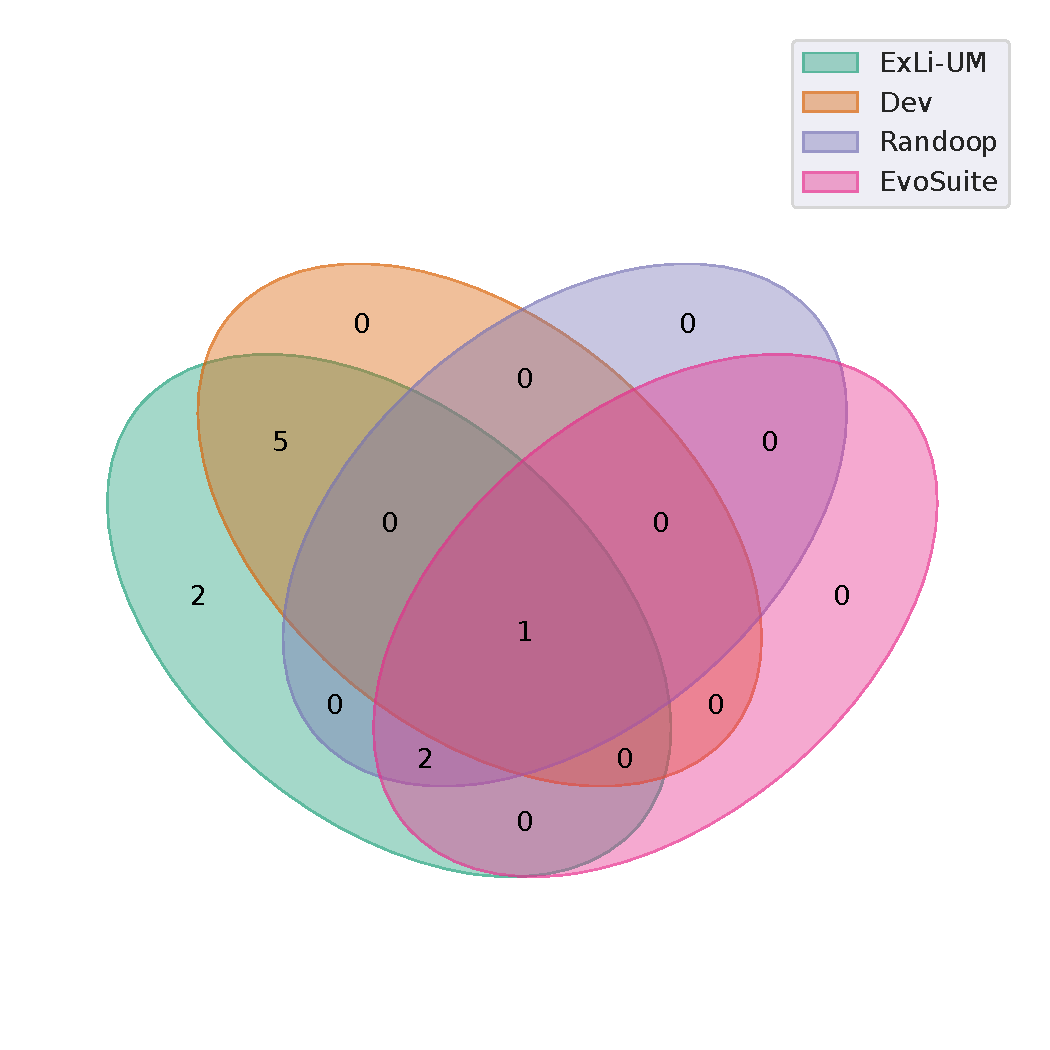
\includegraphics[width=\textwidth]{figures/venn/AquaticInformatics_aquarius-sdk-java-venn.pdf}
\vspace{-10pt}
\caption{aquarius-sdk-java}
\label{fig:venn-AquaticInformatics_aquarius-sdk-java}
\end{subfigure}
\hfill
\begin{subfigure}[b]{0.45\textwidth}
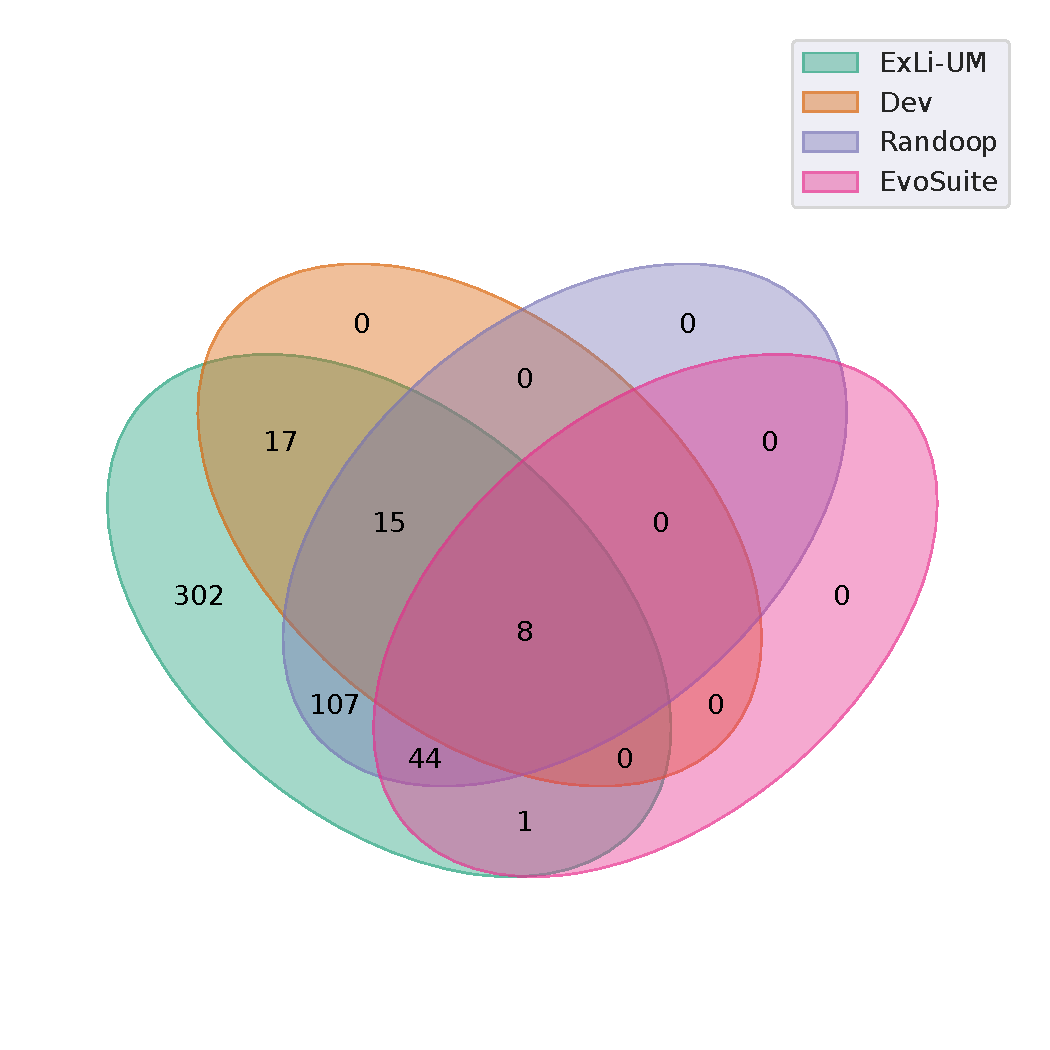
\includegraphics[width=\textwidth]{figures/venn/Asana_java-asana-venn.pdf}
\vspace{-10pt}
\caption{java-asana}
\label{fig:venn-Asana_java-asana}
\end{subfigure}
\end{figure}
\begin{figure}[t]\ContinuedFloat
\begin{subfigure}[b]{0.45\textwidth}
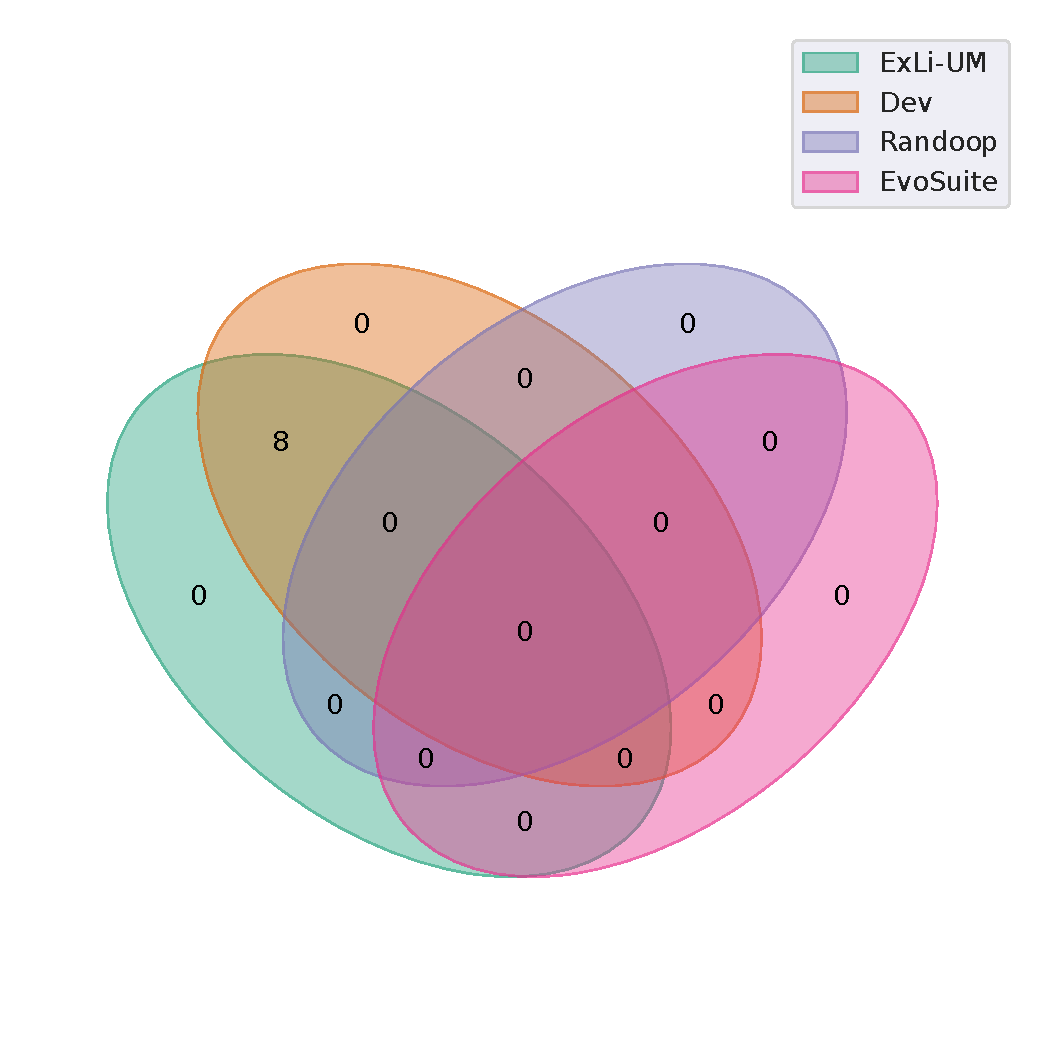
\includegraphics[width=\textwidth]{figures/venn/awslabs_amazon-sqs-java-extended-client-lib-venn.pdf}
\vspace{-10pt}
\caption{amazon-sqs-java-extended-client-lib}
\label{fig:venn-awslabs_amazon-sqs-java-extended-client-lib}
\end{subfigure}
\hfill
\begin{subfigure}[b]{0.45\textwidth}
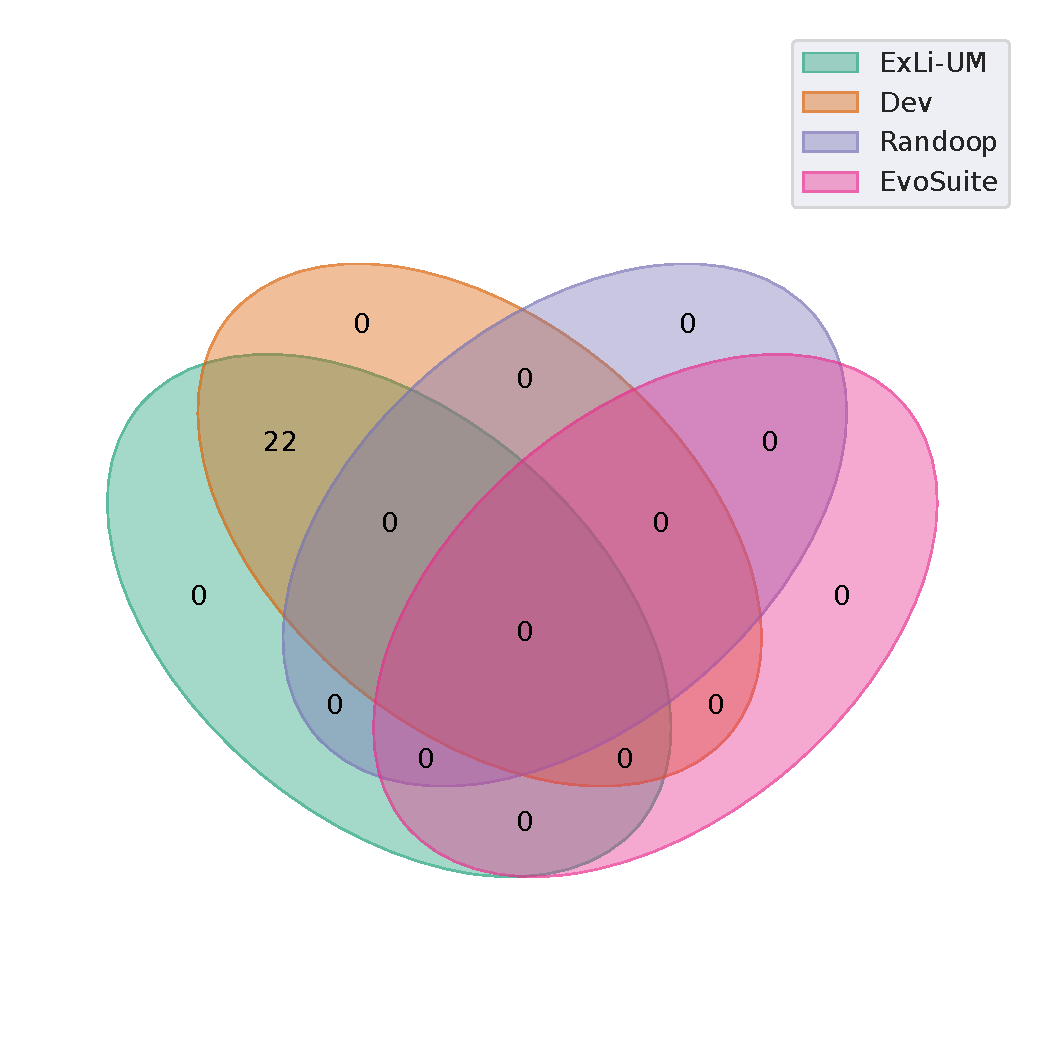
\includegraphics[width=\textwidth]{figures/venn/Bernardo-MG_maven-site-fixer-venn.pdf}
\vspace{-10pt}
\caption{maven-site-fixer}
\label{fig:venn-Bernardo-MG_maven-site-fixer}
\end{subfigure}
\end{figure}
\begin{figure}[t]\ContinuedFloat
\begin{subfigure}[b]{0.45\textwidth}
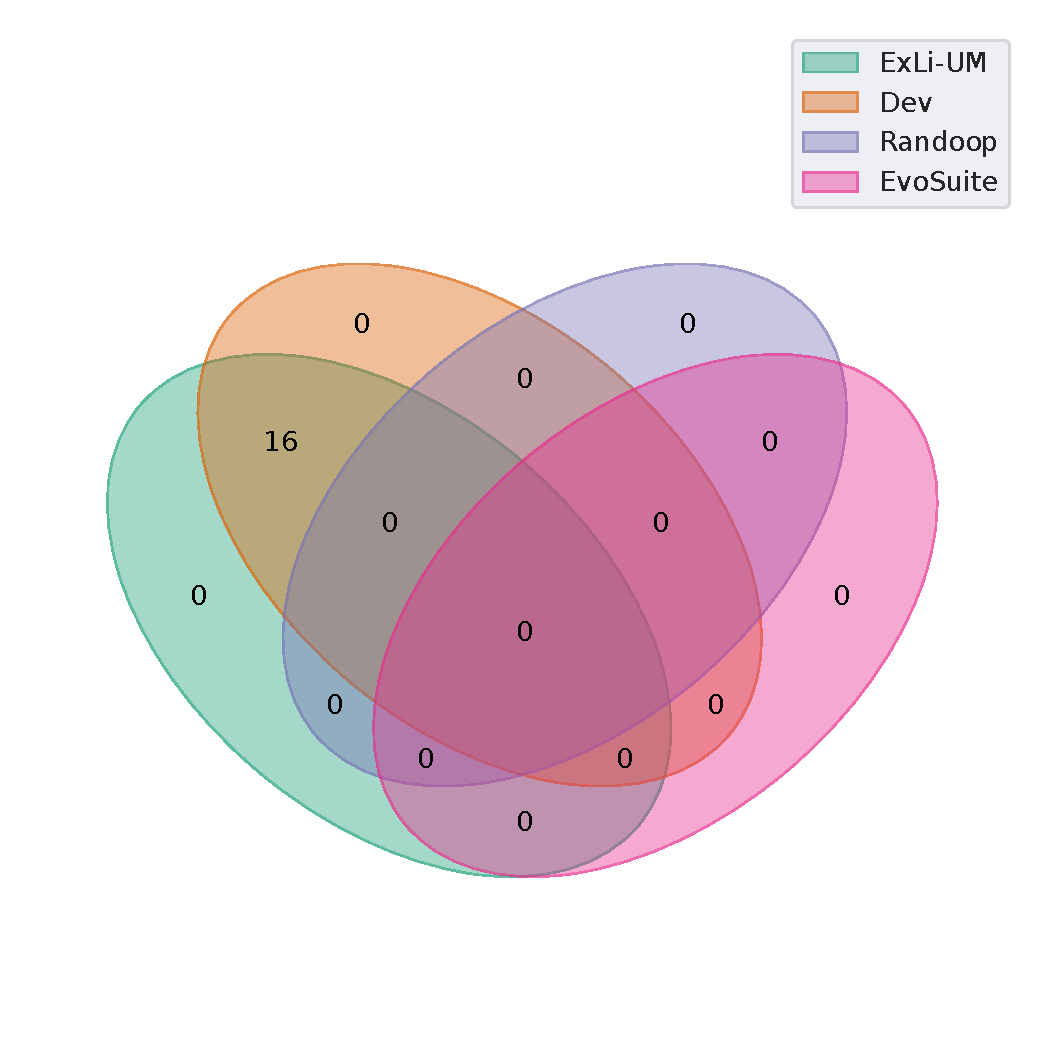
\includegraphics[width=\textwidth]{figures/venn/Bernardo-MG_velocity-config-tool-venn.pdf}
\vspace{-10pt}
\caption{velocity-config-tool}
\label{fig:venn-Bernardo-MG_velocity-config-tool}
\end{subfigure}
\hfill
\begin{subfigure}[b]{0.45\textwidth}
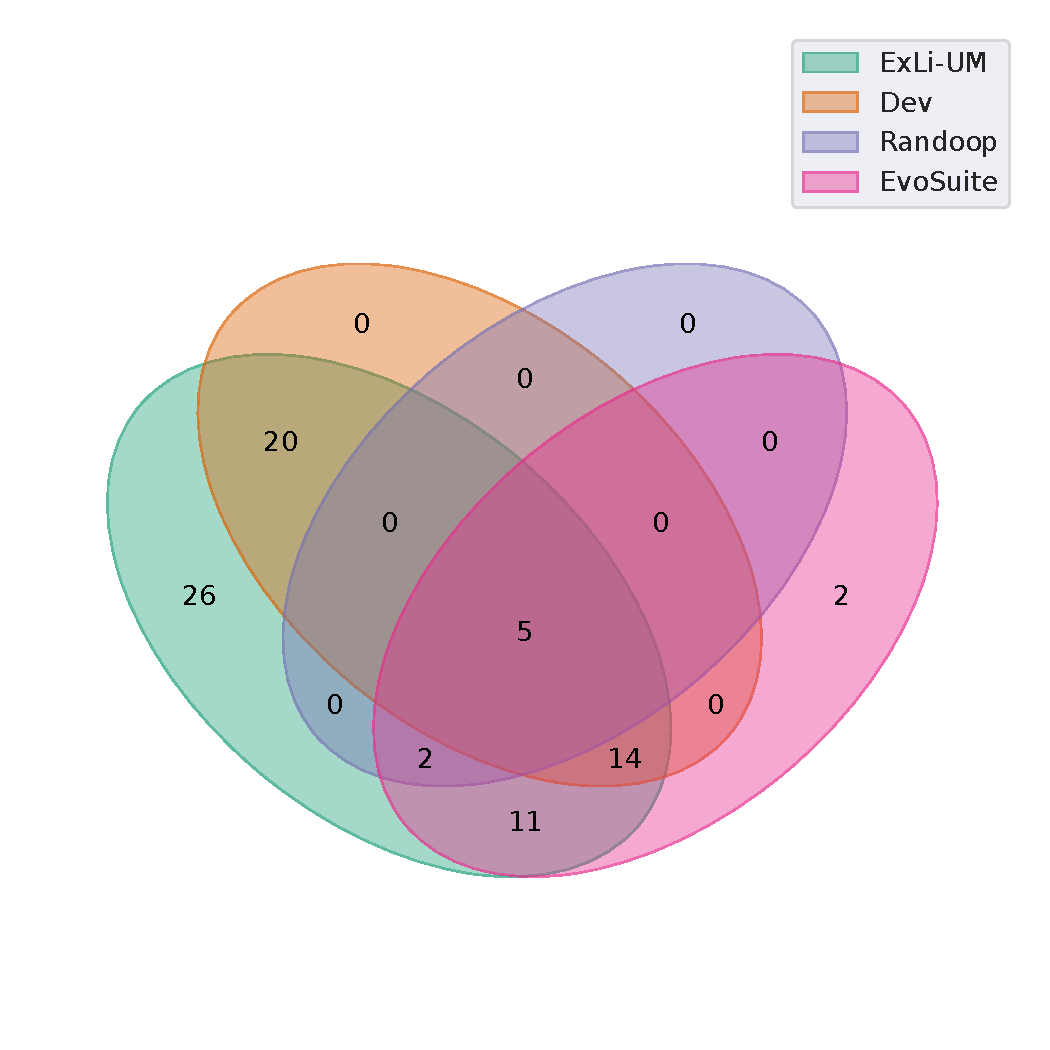
\includegraphics[width=\textwidth]{figures/venn/craftercms_core-venn.pdf}
\vspace{-10pt}
\caption{core}
\label{fig:venn-craftercms_core}
\end{subfigure}
\end{figure}
\begin{figure}[t]\ContinuedFloat
\begin{subfigure}[b]{0.45\textwidth}
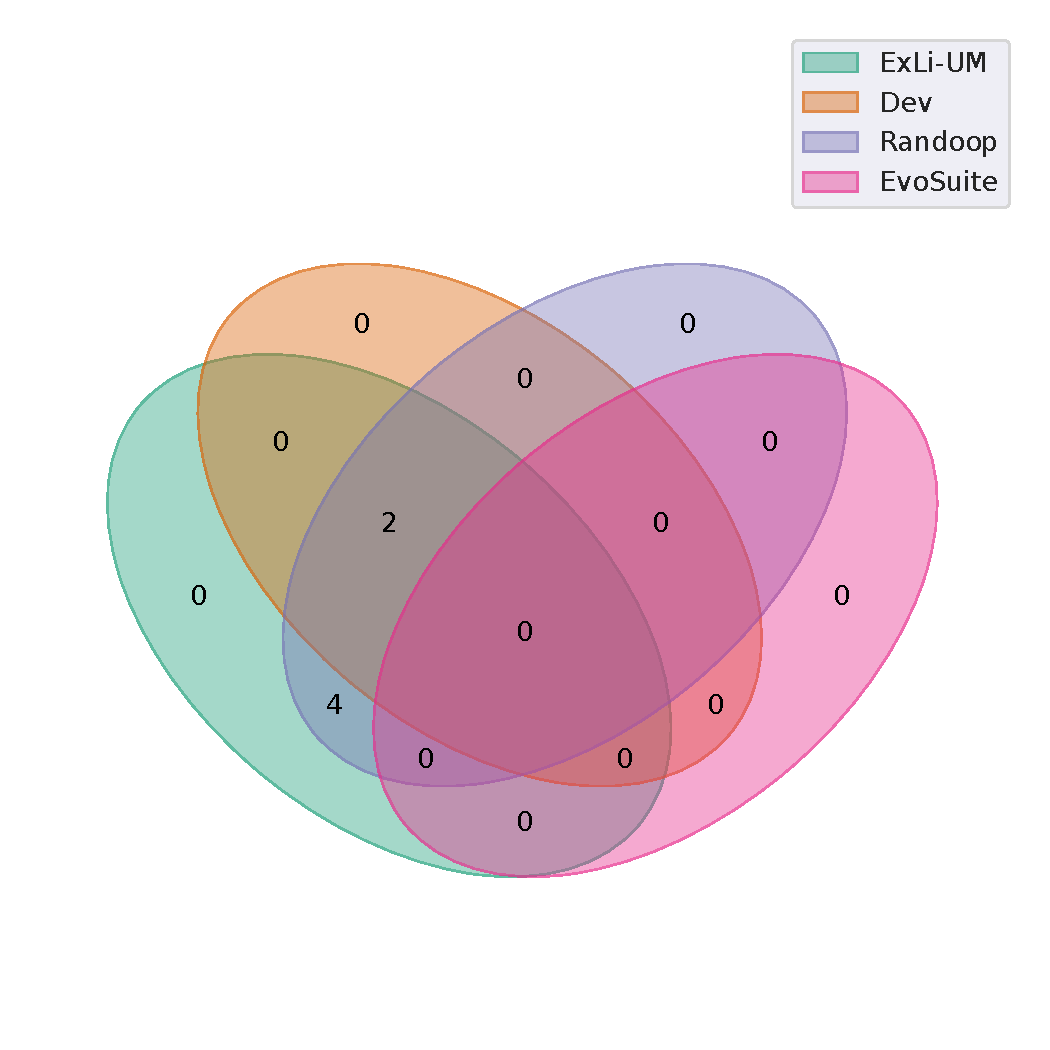
\includegraphics[width=\textwidth]{figures/venn/CycloneDX_cyclonedx-core-java-venn.pdf}
\vspace{-10pt}
\caption{cyclonedx-core-java}
\label{fig:venn-CycloneDX_cyclonedx-core-java}
\end{subfigure}
\hfill
\begin{subfigure}[b]{0.45\textwidth}
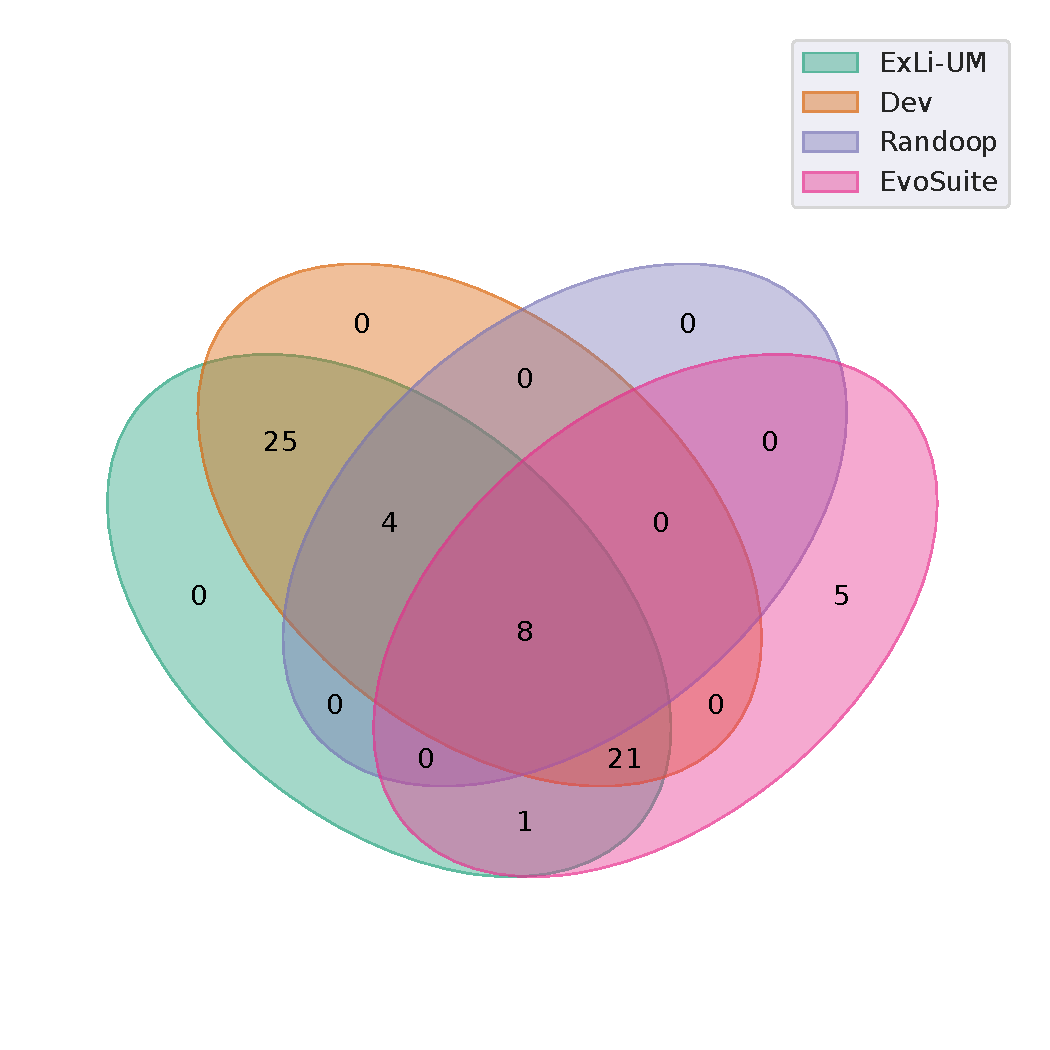
\includegraphics[width=\textwidth]{figures/venn/finos_messageml-utils-venn.pdf}
\vspace{-10pt}
\caption{messageml-utils}
\label{fig:venn-finos_messageml-utils}
\end{subfigure}
\end{figure}
\begin{figure}[t]\ContinuedFloat
\begin{subfigure}[b]{0.45\textwidth}
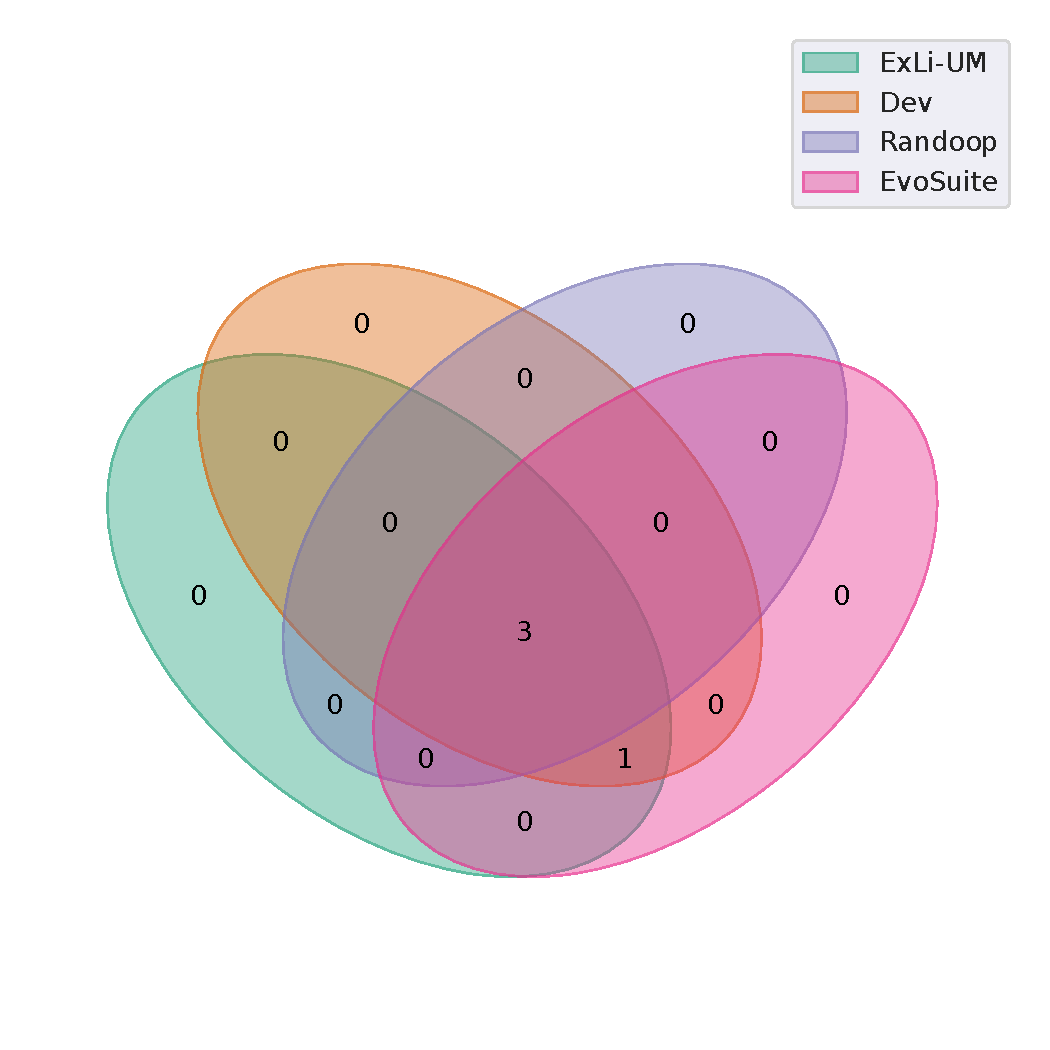
\includegraphics[width=\textwidth]{figures/venn/fleipold_jproc-venn.pdf}
\vspace{-10pt}
\caption{jproc}
\label{fig:venn-fleipold_jproc}
\end{subfigure}
\hfill
\begin{subfigure}[b]{0.45\textwidth}
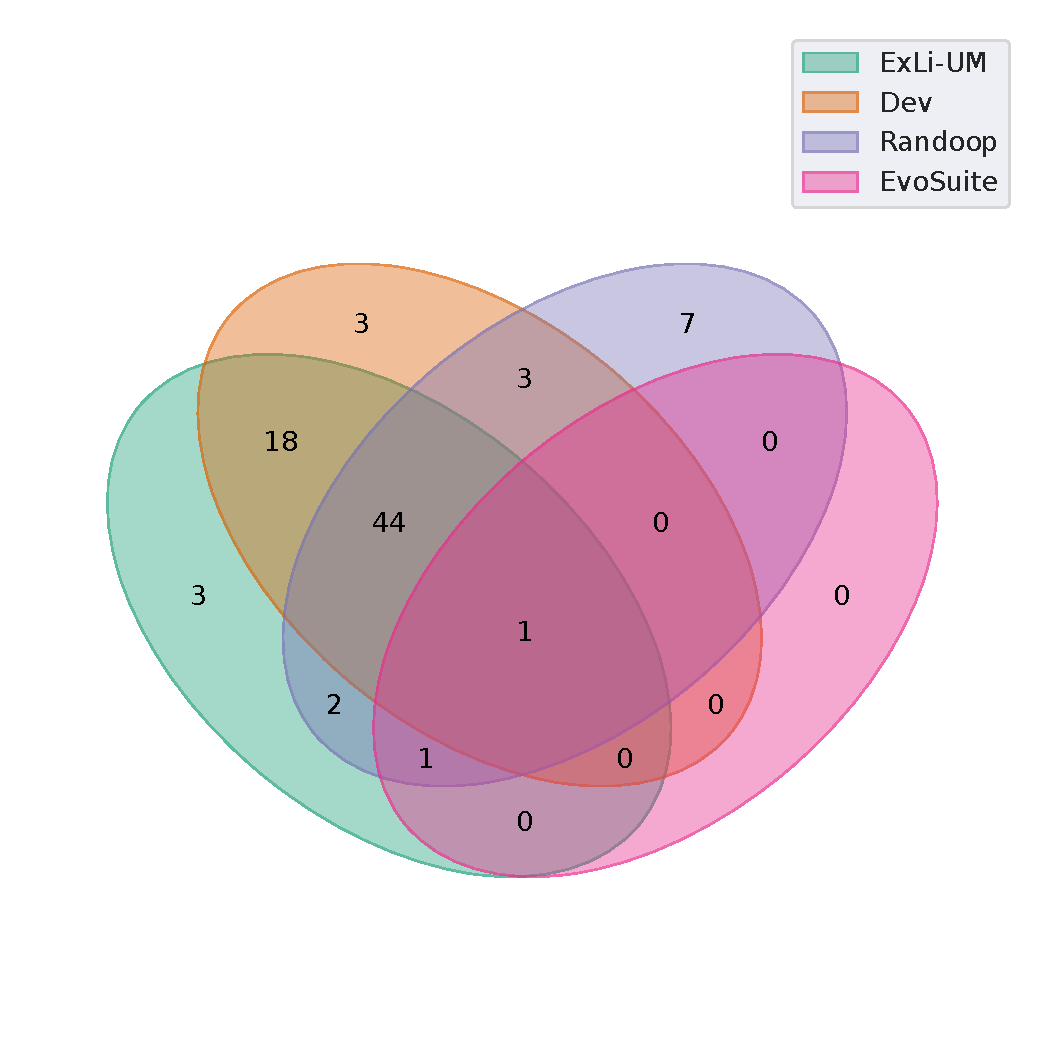
\includegraphics[width=\textwidth]{figures/venn/hyperledger_fabric-sdk-java-venn.pdf}
\vspace{-10pt}
\caption{fabric-sdk-java}
\label{fig:venn-hyperledger_fabric-sdk-java}
\end{subfigure}
\end{figure}
\begin{figure}[t]\ContinuedFloat
\begin{subfigure}[b]{0.45\textwidth}
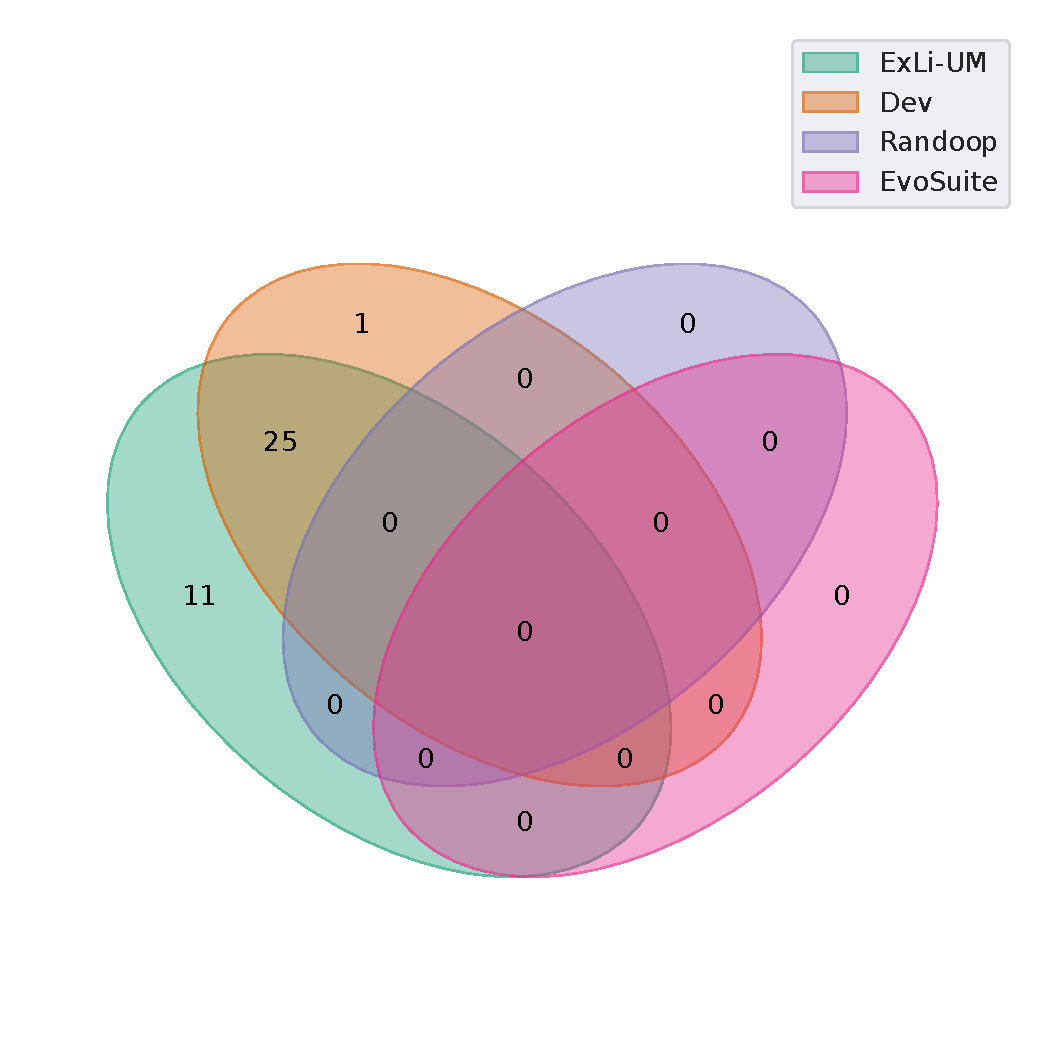
\includegraphics[width=\textwidth]{figures/venn/jenkinsci_email-ext-plugin-venn.pdf}
\vspace{-10pt}
\caption{email-ext-plugin}
\label{fig:venn-jenkinsci_email-ext-plugin}
\end{subfigure}
\hfill
\begin{subfigure}[b]{0.45\textwidth}
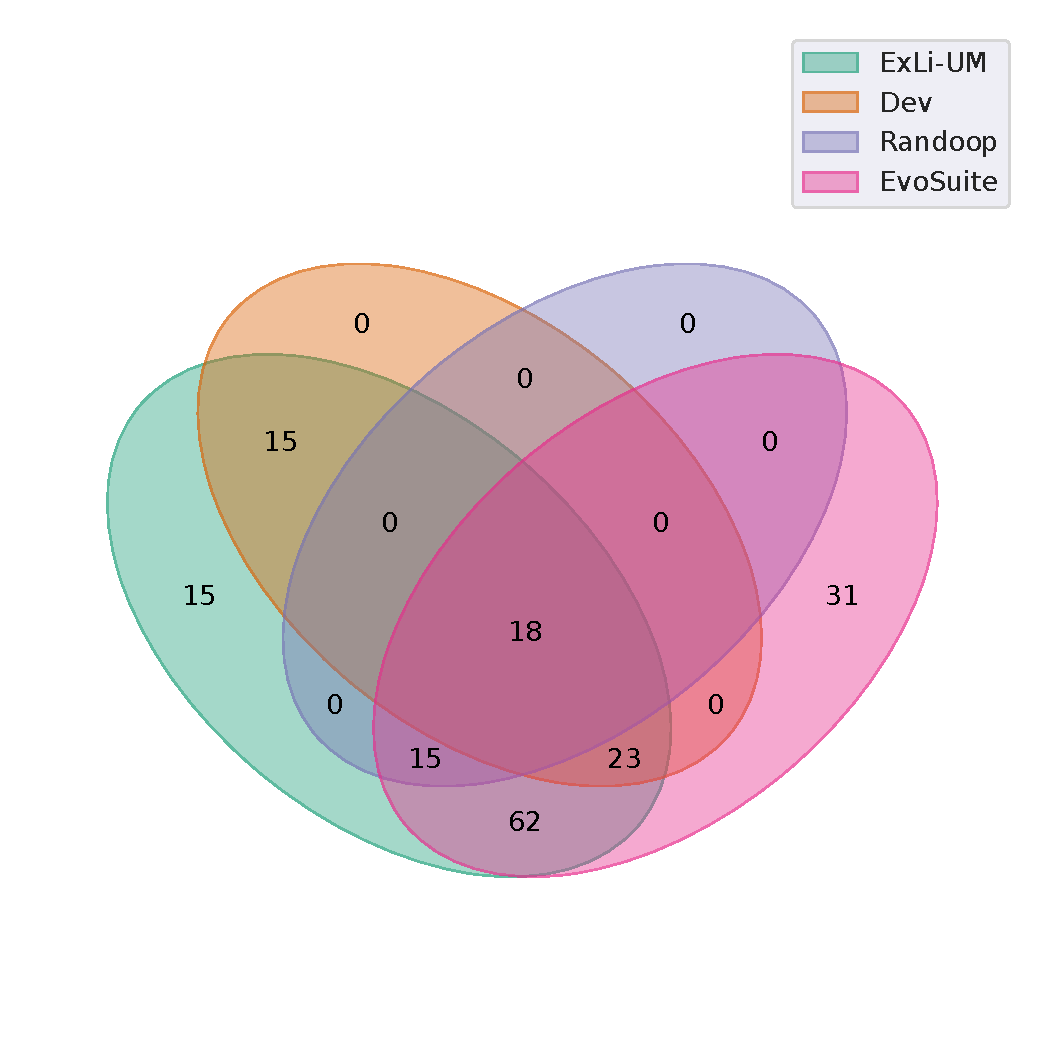
\includegraphics[width=\textwidth]{figures/venn/jkuhnert_ognl-venn.pdf}
\vspace{-10pt}
\caption{ognl}
\label{fig:venn-jkuhnert_ognl}
\end{subfigure}
\end{figure}
\begin{figure}[t]\ContinuedFloat
\begin{subfigure}[b]{0.45\textwidth}
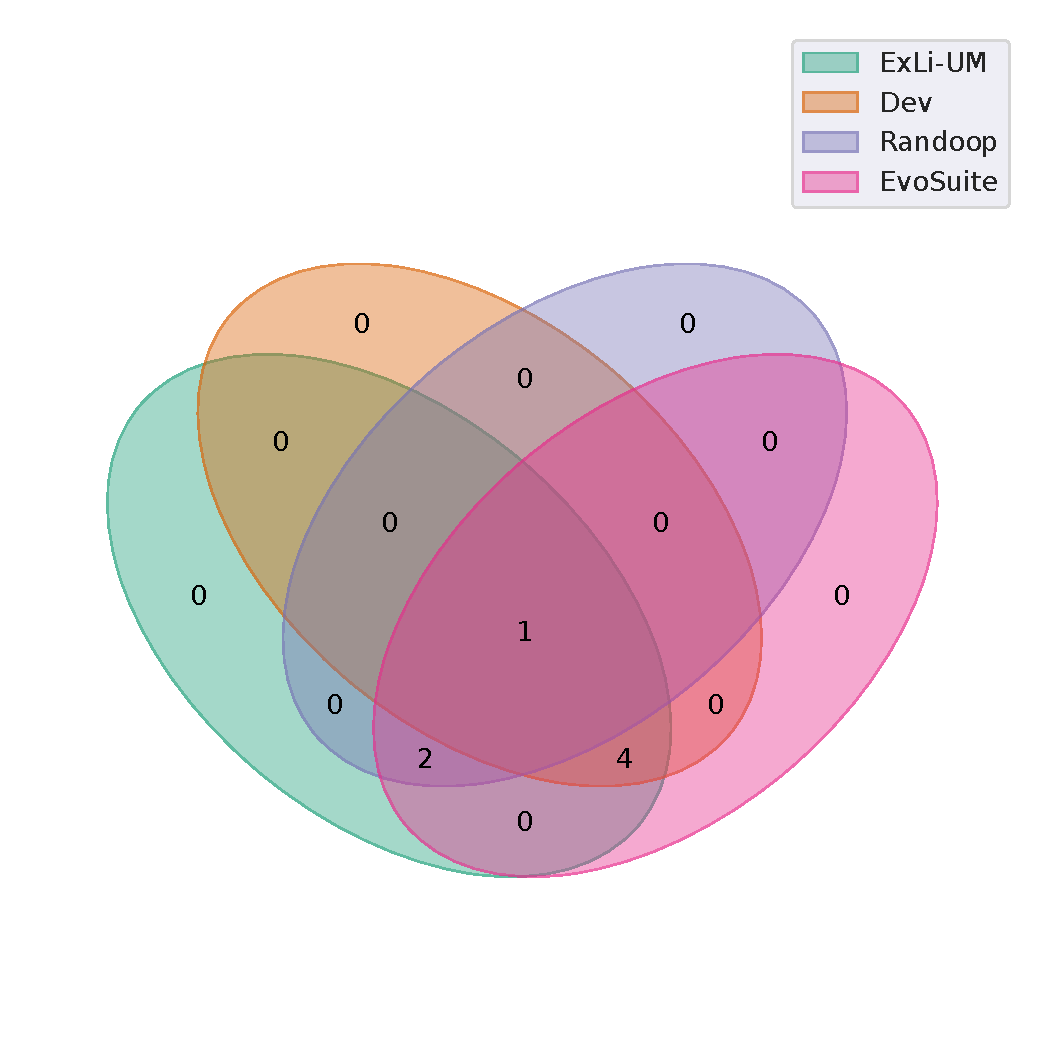
\includegraphics[width=\textwidth]{figures/venn/jscep_jscep-venn.pdf}
\vspace{-10pt}
\caption{jscep}
\label{fig:venn-jscep_jscep}
\end{subfigure}
\hfill
\begin{subfigure}[b]{0.45\textwidth}
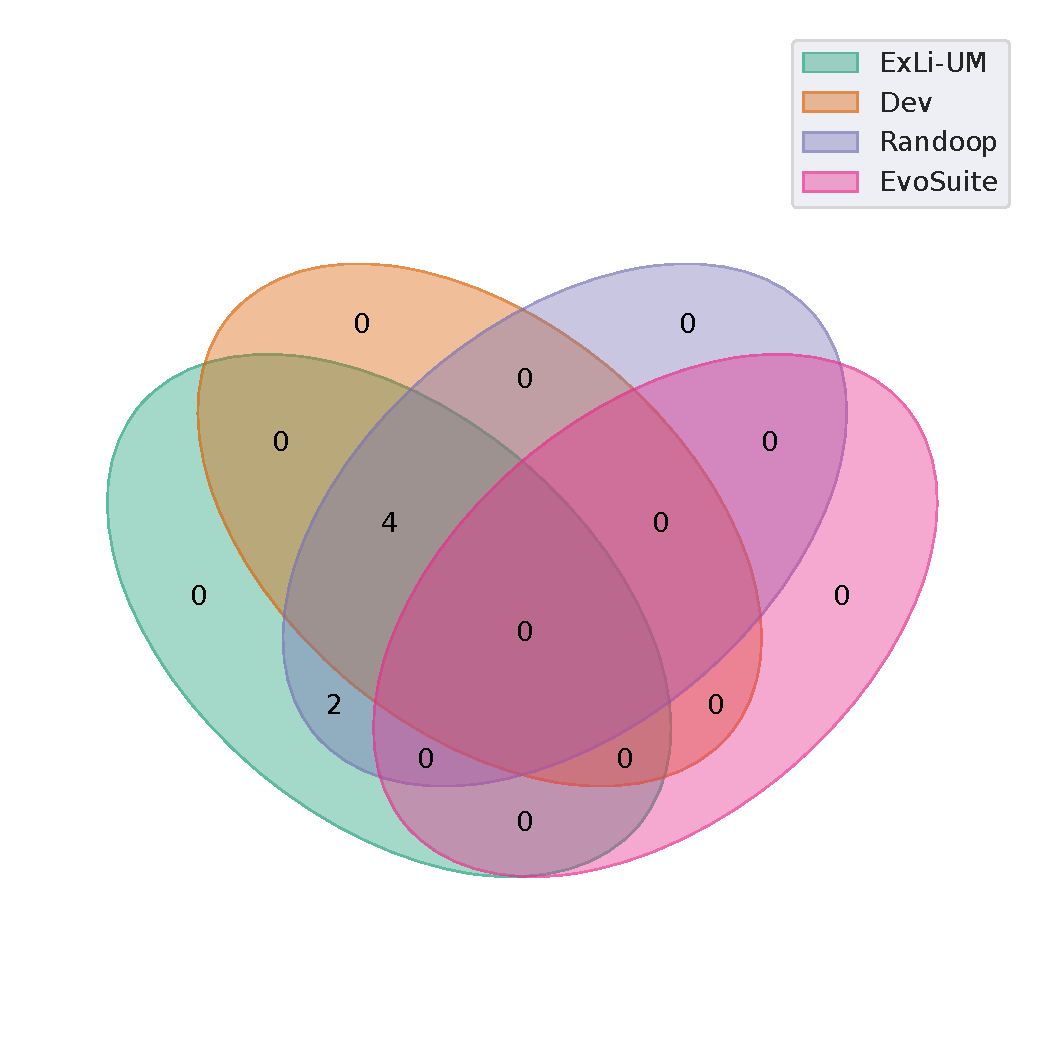
\includegraphics[width=\textwidth]{figures/venn/lamarios_sherdog-parser-venn.pdf}
\vspace{-10pt}
\caption{sherdog-parser}
\label{fig:venn-lamarios_sherdog-parser}
\end{subfigure}
\end{figure}
\begin{figure}[t]\ContinuedFloat
\begin{subfigure}[b]{0.45\textwidth}
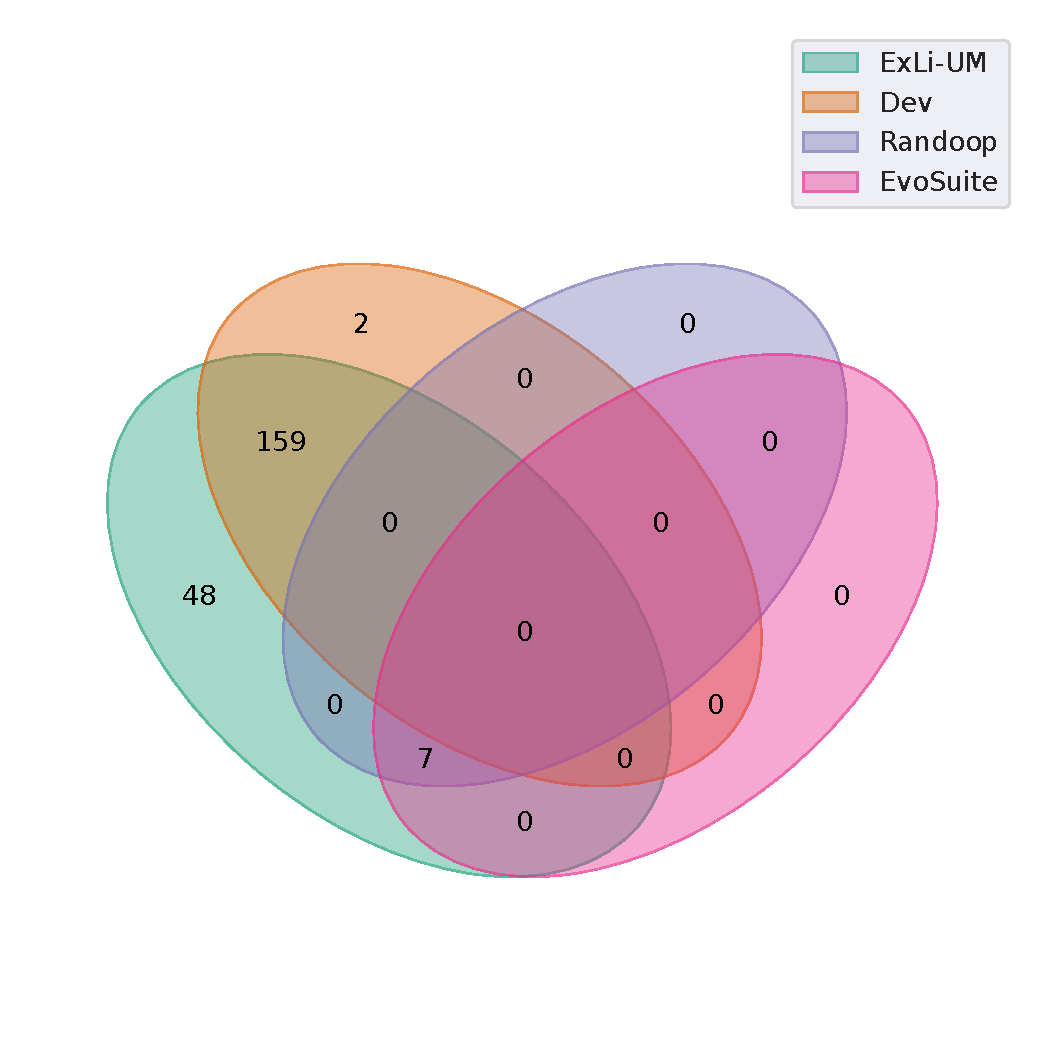
\includegraphics[width=\textwidth]{figures/venn/maxmind_geoip-api-java-venn.pdf}
\vspace{-10pt}
\caption{geoip-api-java}
\label{fig:venn-maxmind_geoip-api-java}
\end{subfigure}
\hfill
\begin{subfigure}[b]{0.45\textwidth}
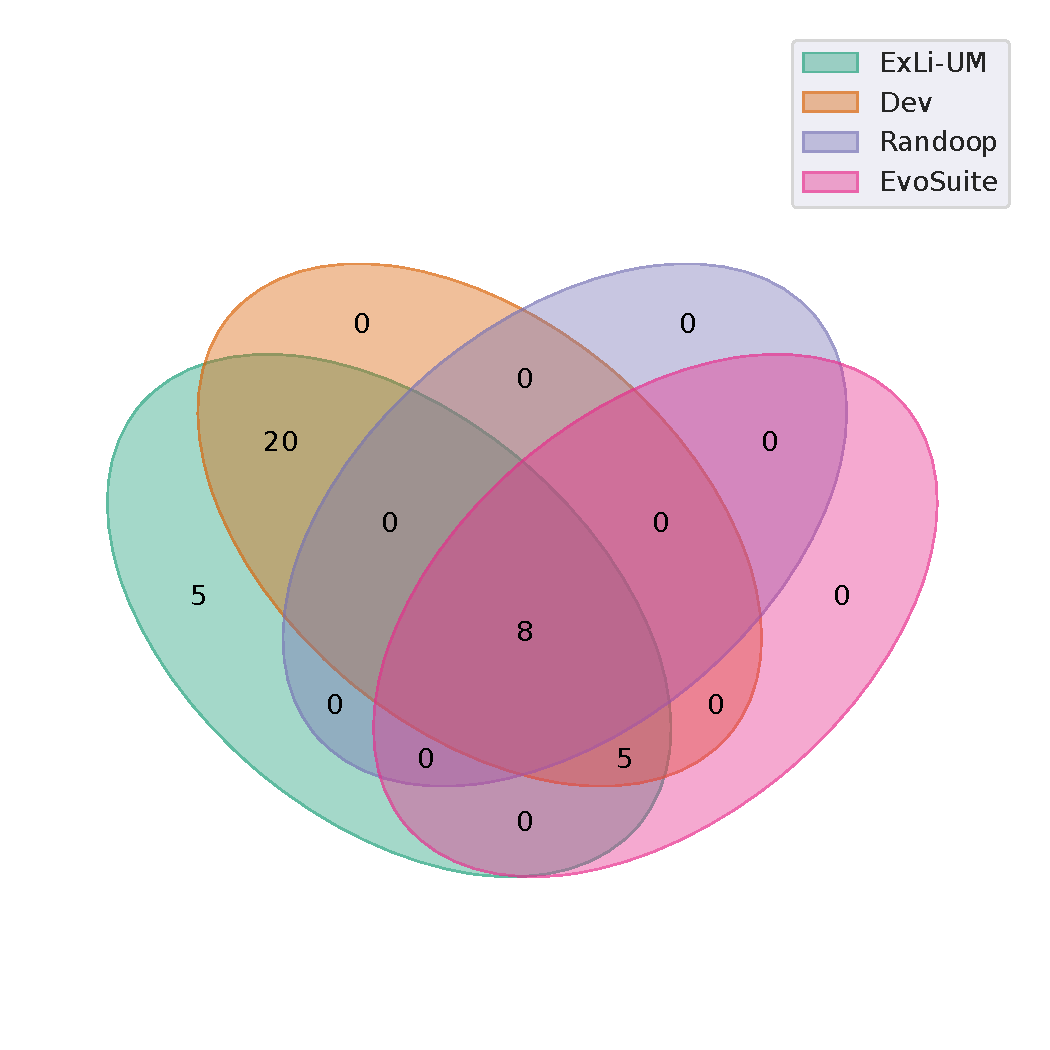
\includegraphics[width=\textwidth]{figures/venn/medcl_elasticsearch-analysis-pinyin-venn.pdf}
\vspace{-10pt}
\caption{elasticsearch-analysis-pinyin}
\label{fig:venn-medcl_elasticsearch-analysis-pinyin}
\end{subfigure}
\end{figure}
\begin{figure}[t]\ContinuedFloat
\begin{subfigure}[b]{0.45\textwidth}
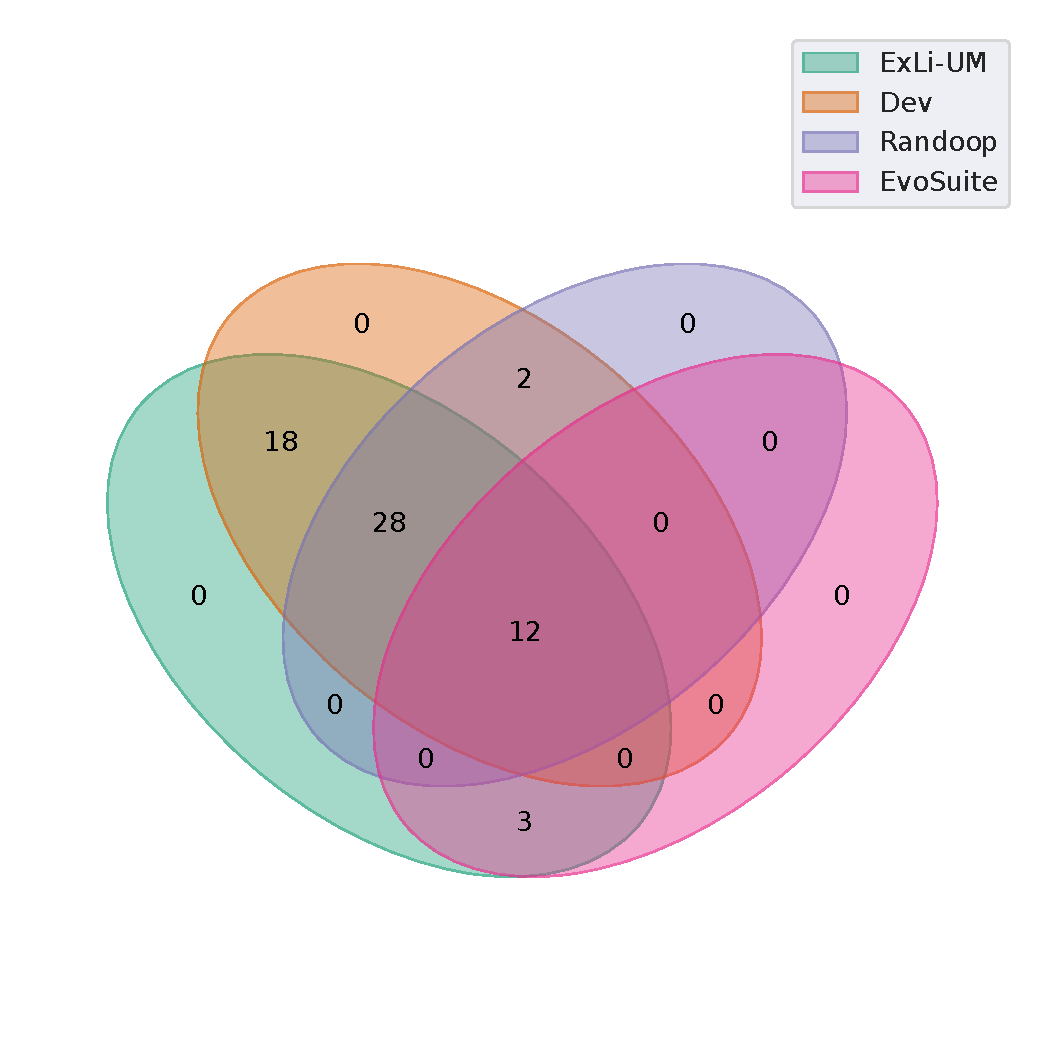
\includegraphics[width=\textwidth]{figures/venn/mojohaus_build-helper-maven-plugin-venn.pdf}
\vspace{-10pt}
\caption{build-helper-maven-plugin}
\label{fig:venn-mojohaus_build-helper-maven-plugin}
\end{subfigure}
\hfill
\begin{subfigure}[b]{0.45\textwidth}
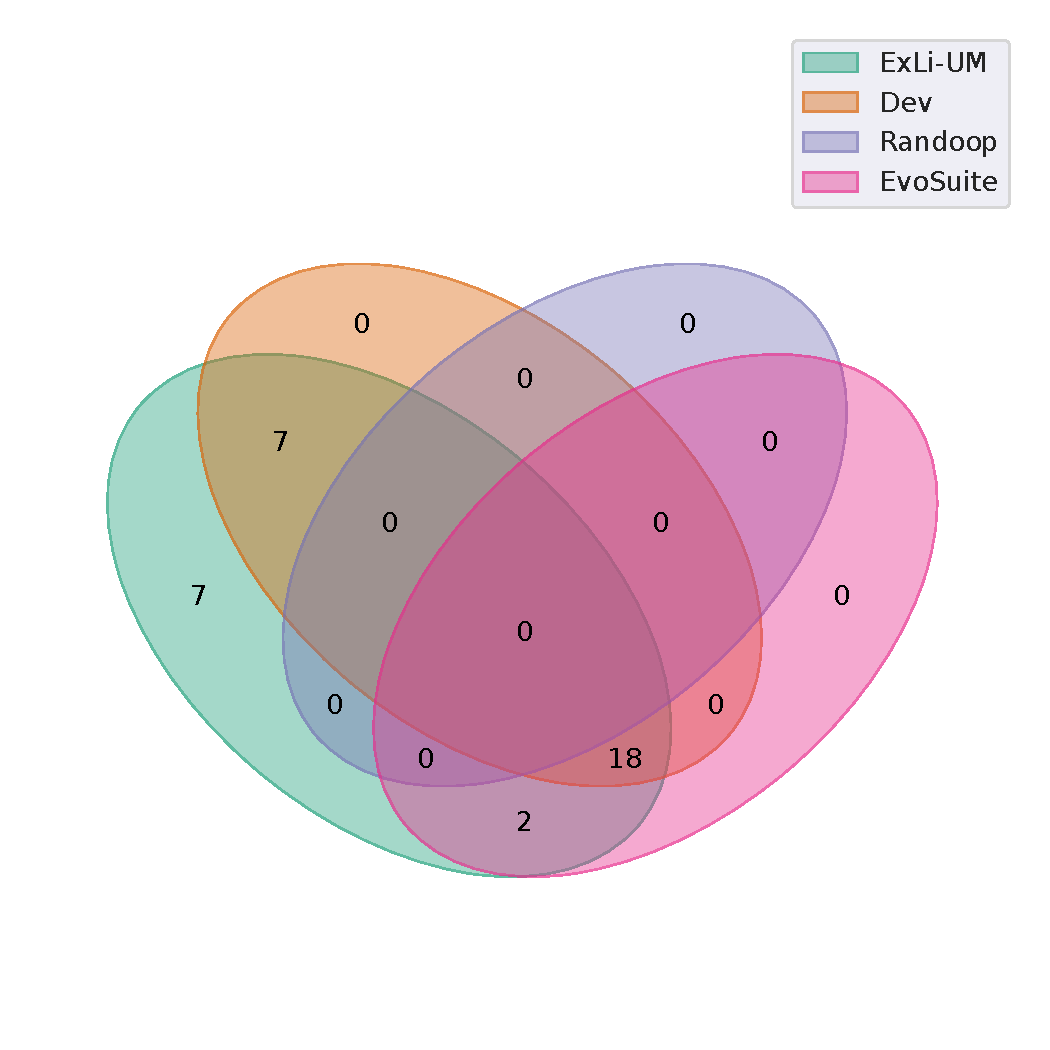
\includegraphics[width=\textwidth]{figures/venn/mojohaus_properties-maven-plugin-venn.pdf}
\vspace{-10pt}
\caption{properties-maven-plugin}
\label{fig:venn-mojohaus_properties-maven-plugin}
\end{subfigure}
\end{figure}
\begin{figure}[t]\ContinuedFloat
\begin{subfigure}[b]{0.45\textwidth}
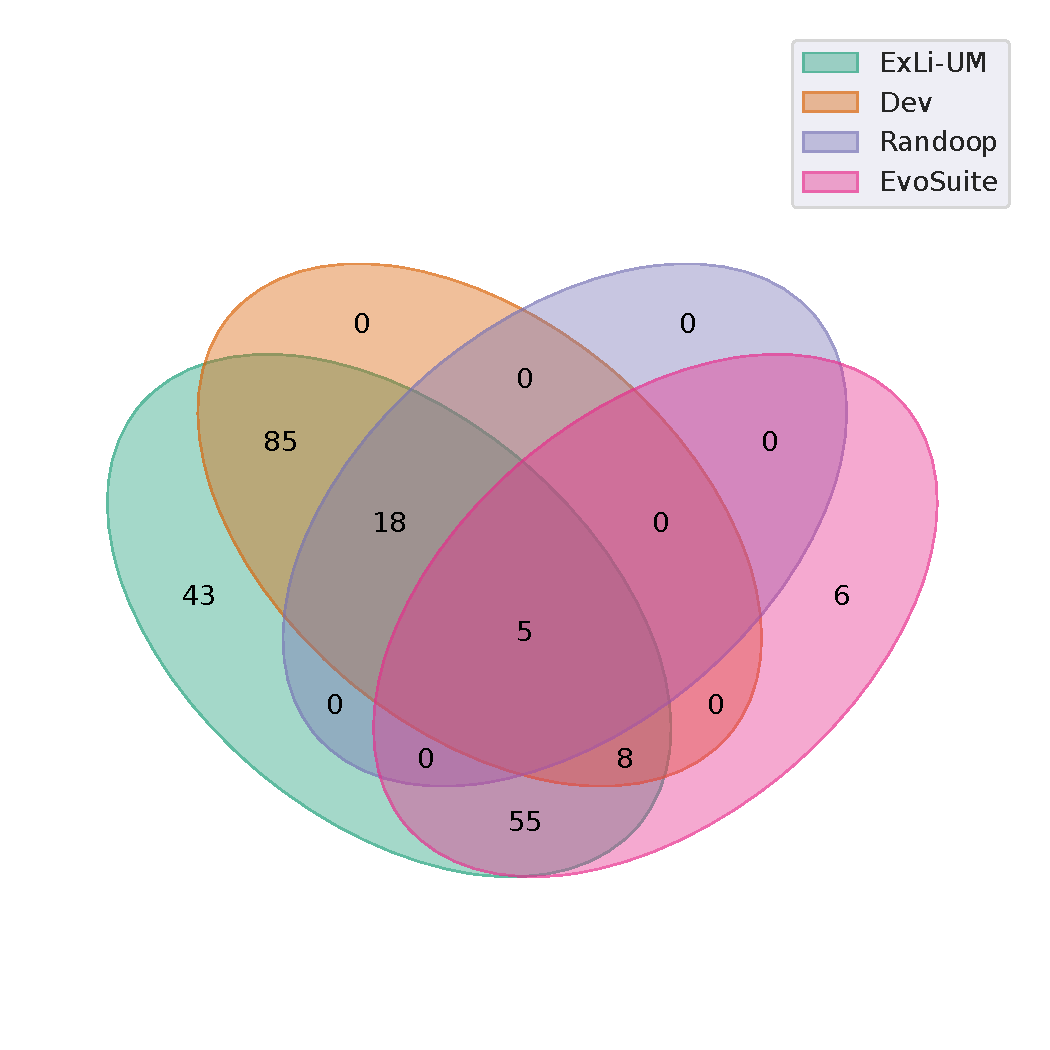
\includegraphics[width=\textwidth]{figures/venn/mp911de_logstash-gelf-venn.pdf}
\vspace{-10pt}
\caption{logstash-gelf}
\label{fig:venn-mp911de_logstash-gelf}
\end{subfigure}
\hfill
\begin{subfigure}[b]{0.45\textwidth}
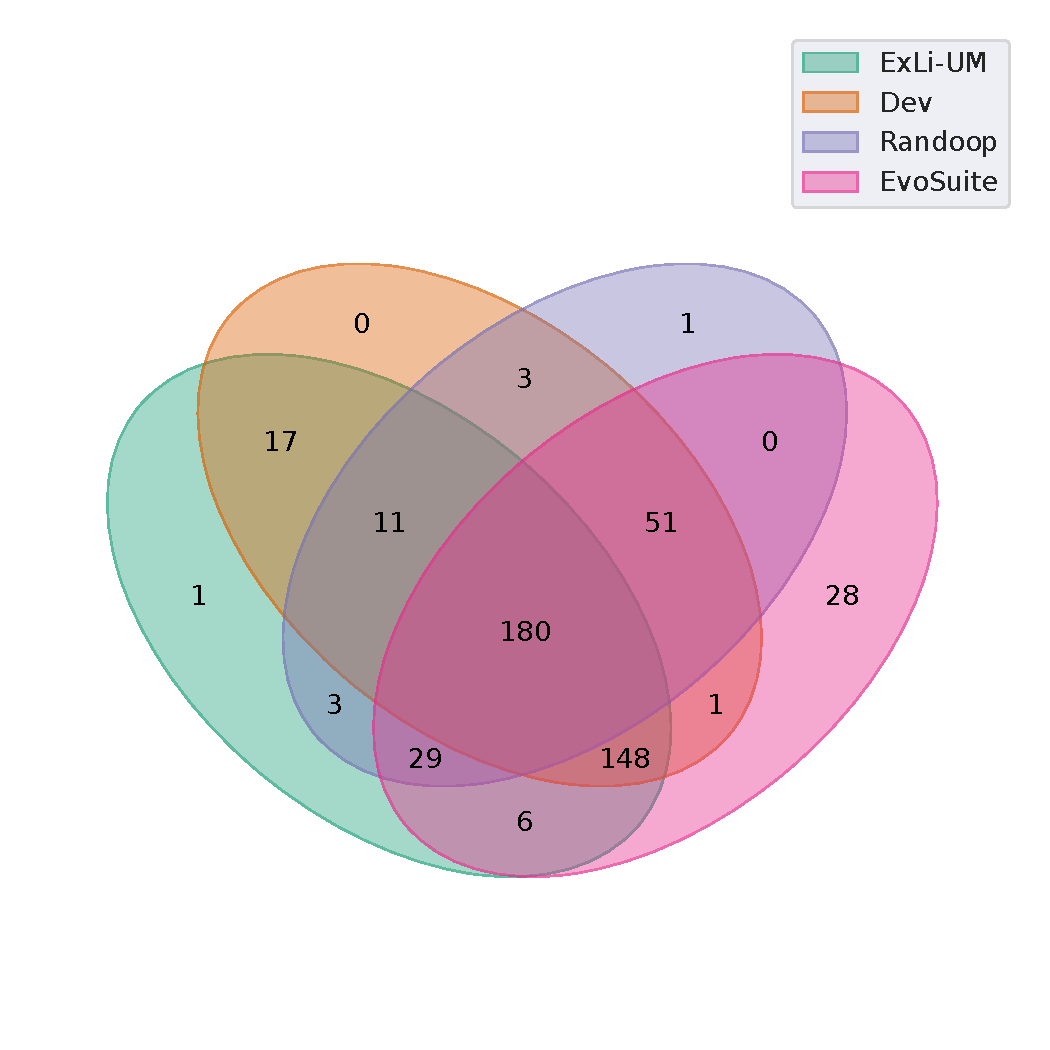
\includegraphics[width=\textwidth]{figures/venn/mpatric_mp3agic-venn.pdf}
\vspace{-10pt}
\caption{mp3agic}
\label{fig:venn-mpatric_mp3agic}
\end{subfigure}
\end{figure}
\begin{figure}[t]\ContinuedFloat
\begin{subfigure}[b]{0.45\textwidth}
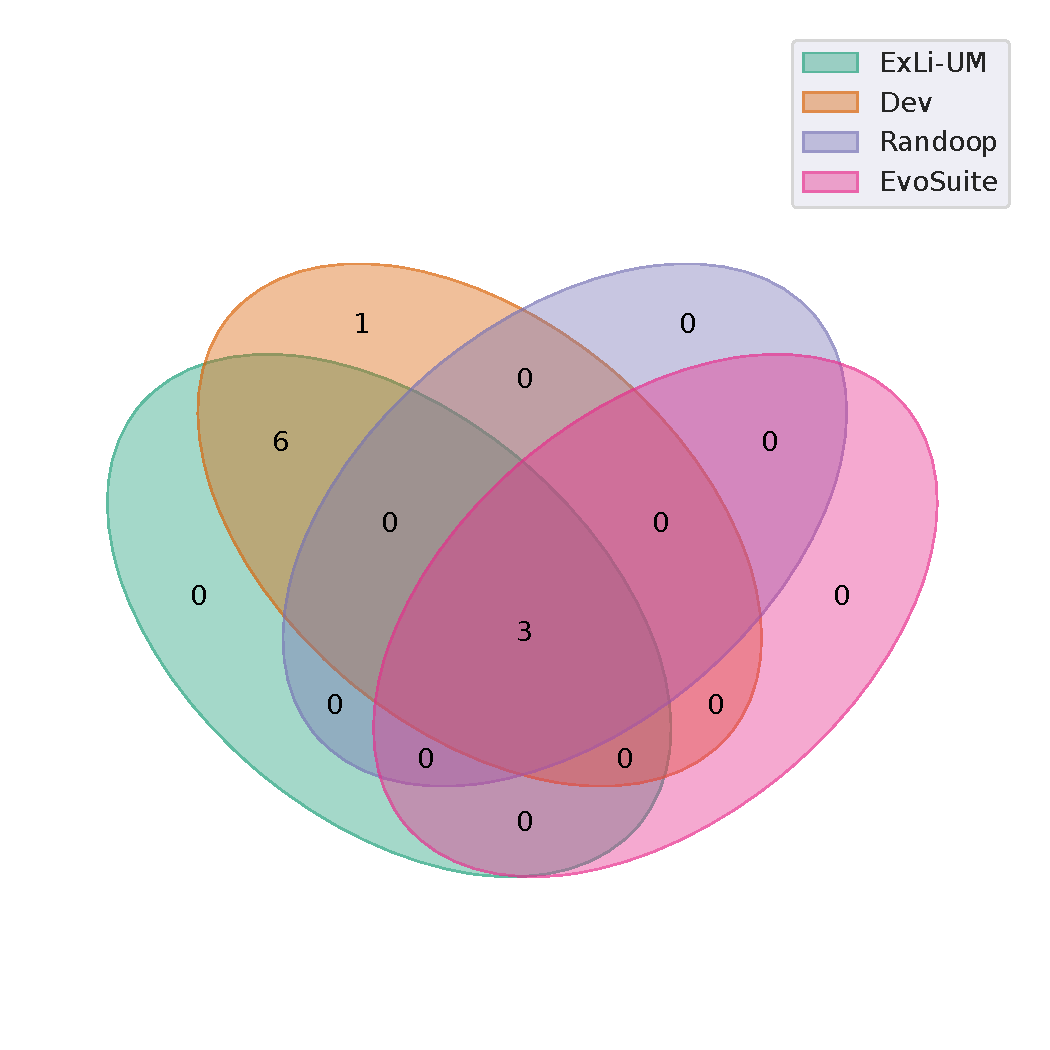
\includegraphics[width=\textwidth]{figures/venn/netceteragroup_trema-core-venn.pdf}
\vspace{-10pt}
\caption{trema-core}
\label{fig:venn-netceteragroup_trema-core}
\end{subfigure}
\hfill
\begin{subfigure}[b]{0.45\textwidth}
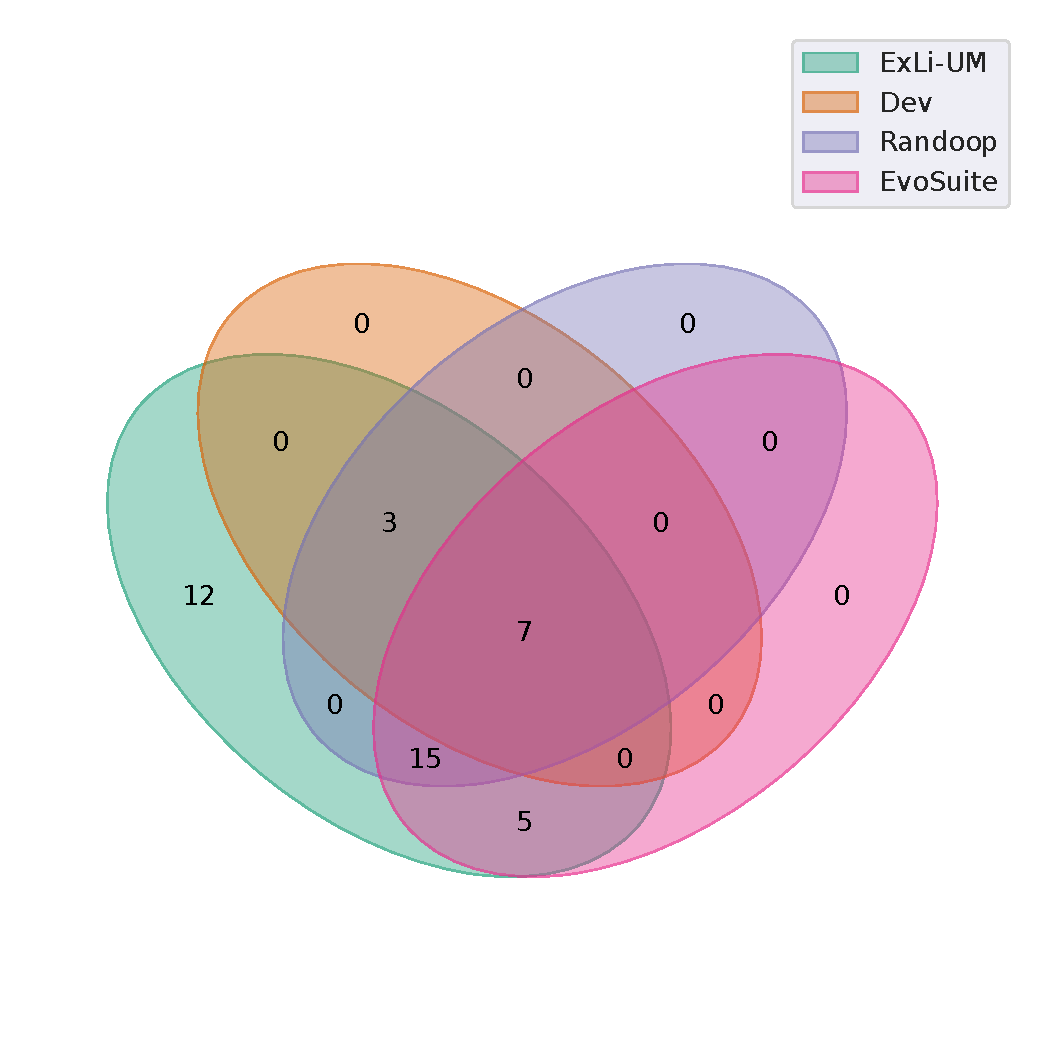
\includegraphics[width=\textwidth]{figures/venn/phax_ph-pdf-layout-venn.pdf}
\vspace{-10pt}
\caption{ph-pdf-layout}
\label{fig:venn-phax_ph-pdf-layout}
\end{subfigure}
\end{figure}
\begin{figure}[t]\ContinuedFloat
\begin{subfigure}[b]{0.45\textwidth}
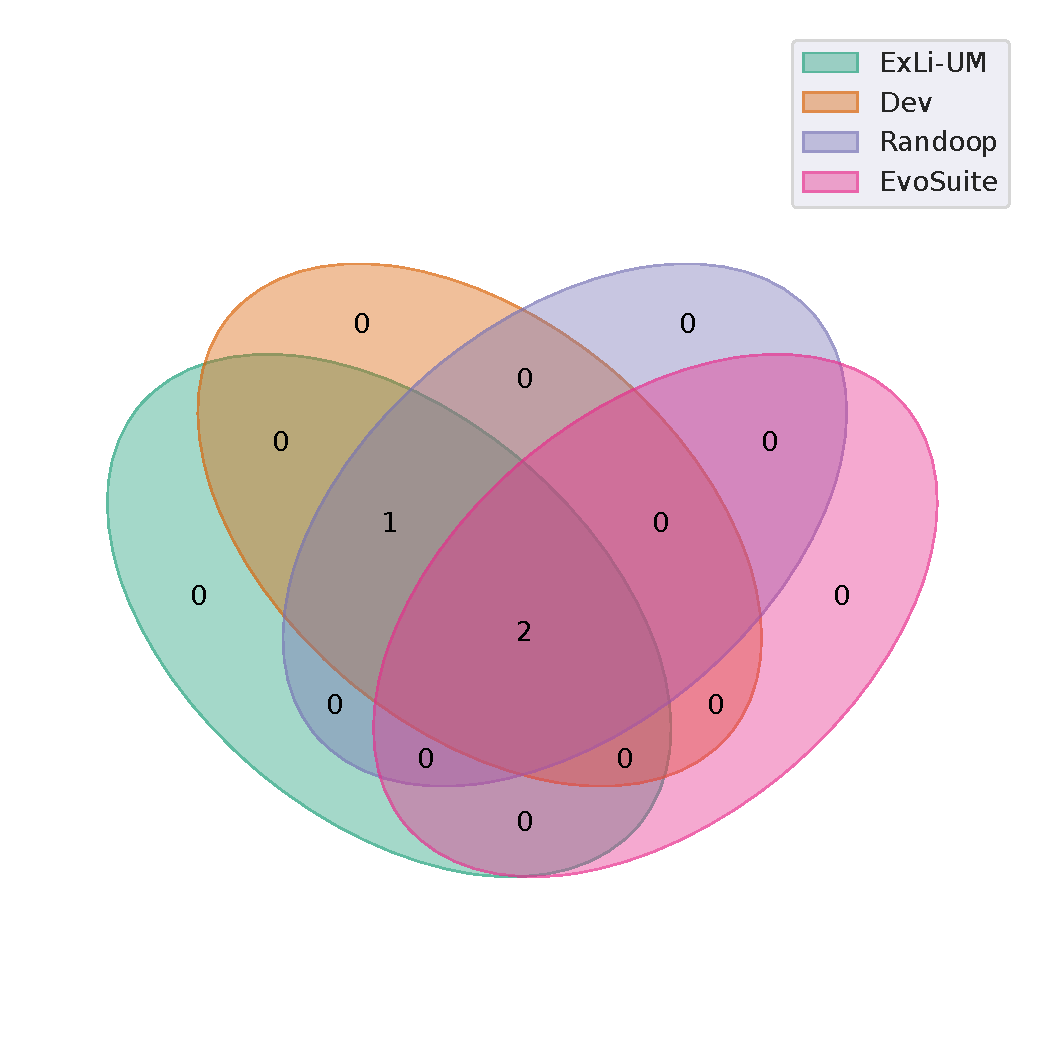
\includegraphics[width=\textwidth]{figures/venn/ralscha_extclassgenerator-venn.pdf}
\vspace{-10pt}
\caption{extclassgenerator}
\label{fig:venn-ralscha_extclassgenerator}
\end{subfigure}
\hfill
\begin{subfigure}[b]{0.45\textwidth}
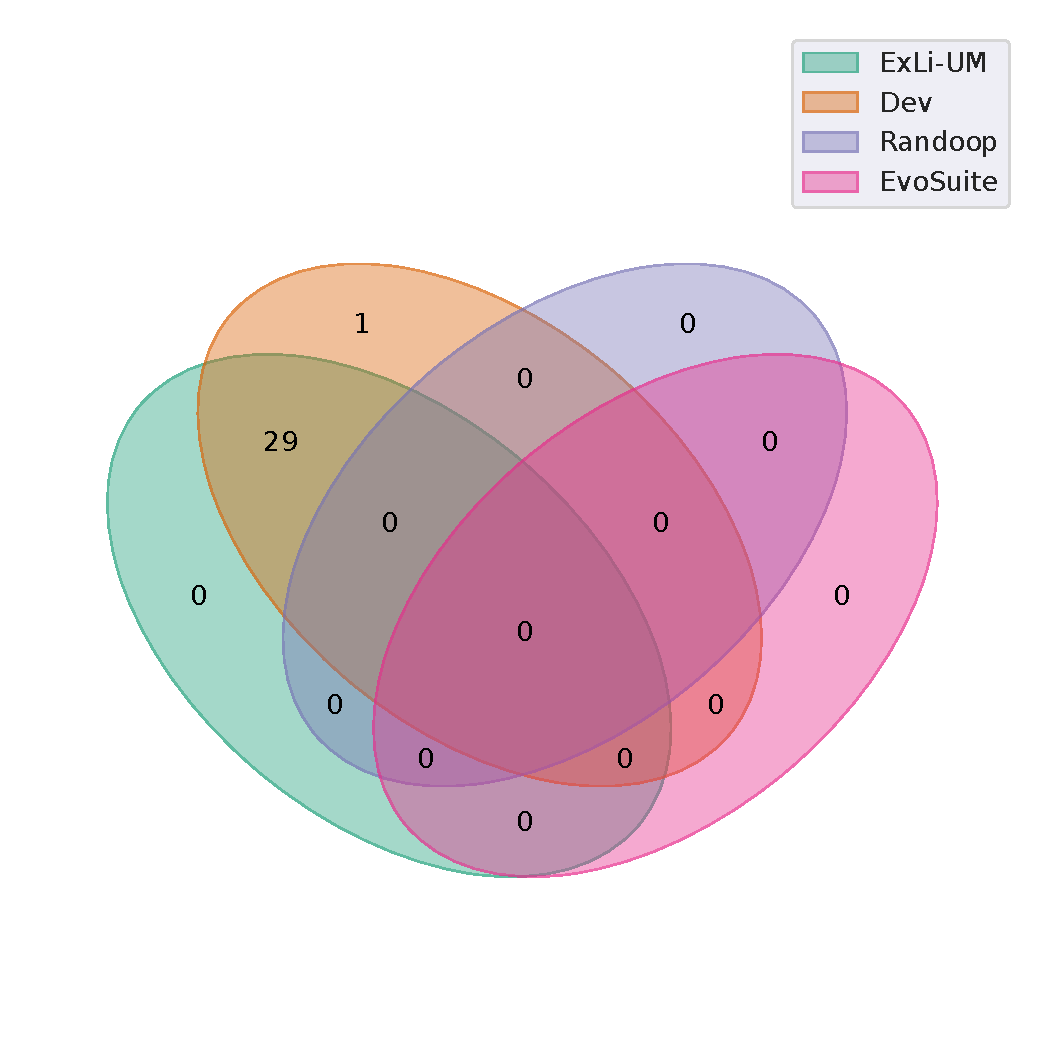
\includegraphics[width=\textwidth]{figures/venn/red6_pdfcompare-venn.pdf}
\vspace{-10pt}
\caption{pdfcompare}
\label{fig:venn-red6_pdfcompare}
\end{subfigure}
\end{figure}
\begin{figure}[t]\ContinuedFloat
\begin{subfigure}[b]{0.45\textwidth}
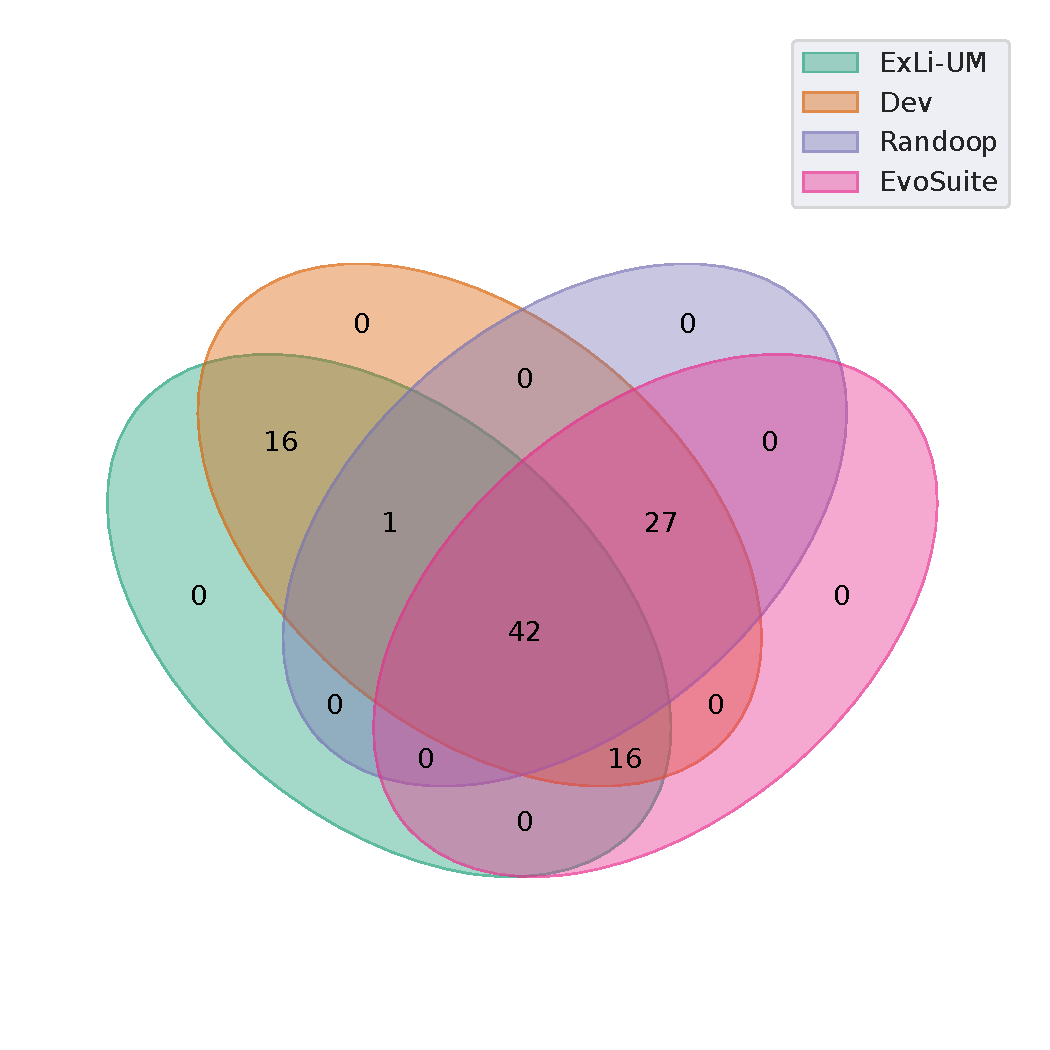
\includegraphics[width=\textwidth]{figures/venn/restfb_restfb-venn.pdf}
\vspace{-10pt}
\caption{restfb}
\label{fig:venn-restfb_restfb}
\end{subfigure}
\hfill
\begin{subfigure}[b]{0.45\textwidth}
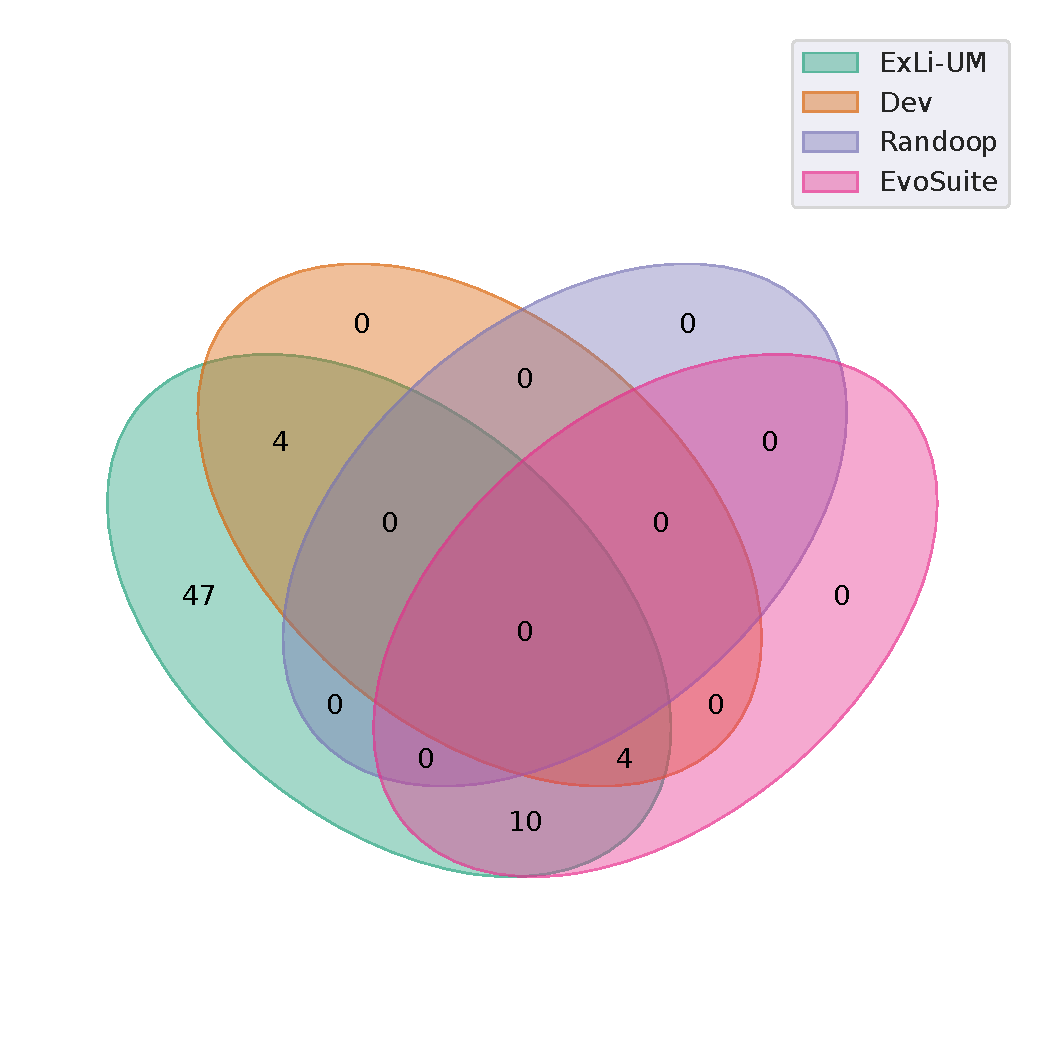
\includegraphics[width=\textwidth]{figures/venn/steveash_jopenfst-venn.pdf}
\vspace{-10pt}
\caption{jopenfst}
\label{fig:venn-steveash_jopenfst}
\end{subfigure}
\end{figure}
\begin{figure}[t]\ContinuedFloat
\begin{subfigure}[b]{0.45\textwidth}
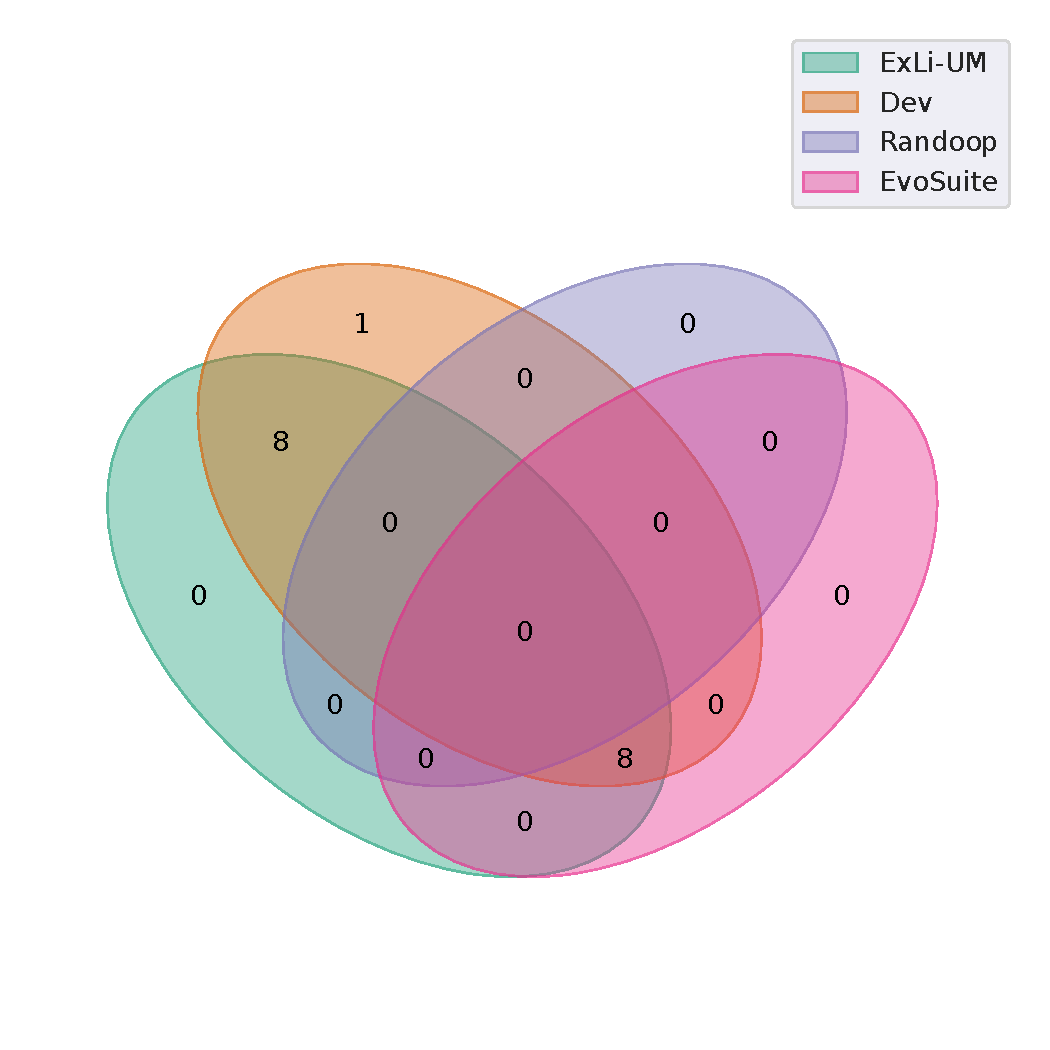
\includegraphics[width=\textwidth]{figures/venn/TNG_property-loader-venn.pdf}
\vspace{-10pt}
\caption{property-loader}
\label{fig:venn-TNG_property-loader}
\end{subfigure}
\hfill
\begin{subfigure}[b]{0.45\textwidth}
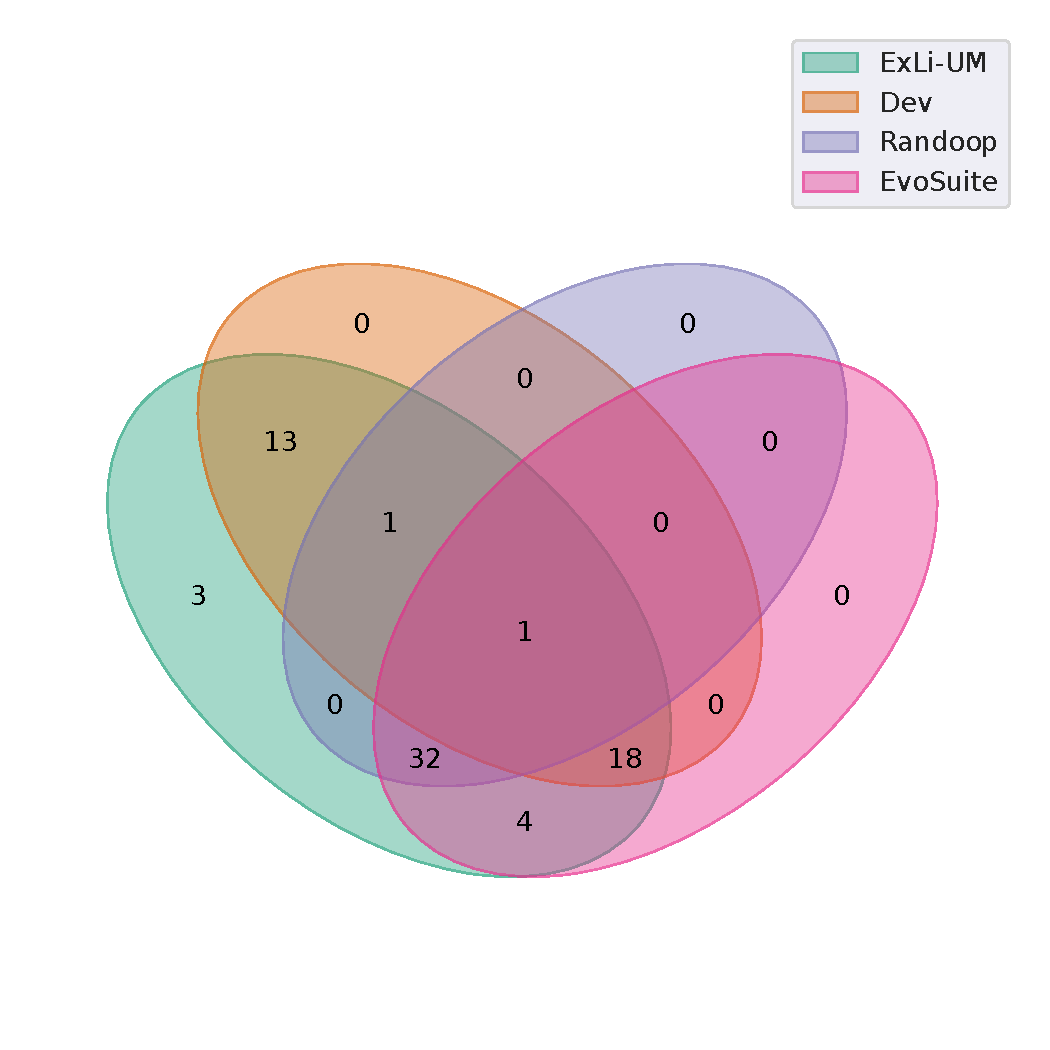
\includegraphics[width=\textwidth]{figures/venn/uwolfer_gerrit-rest-java-client-venn.pdf}
\vspace{-10pt}
\caption{gerrit-rest-java-client}
\label{fig:venn-uwolfer_gerrit-rest-java-client}
\end{subfigure}
\end{figure}
\begin{figure}[t]\ContinuedFloat
\begin{subfigure}[b]{0.45\textwidth}
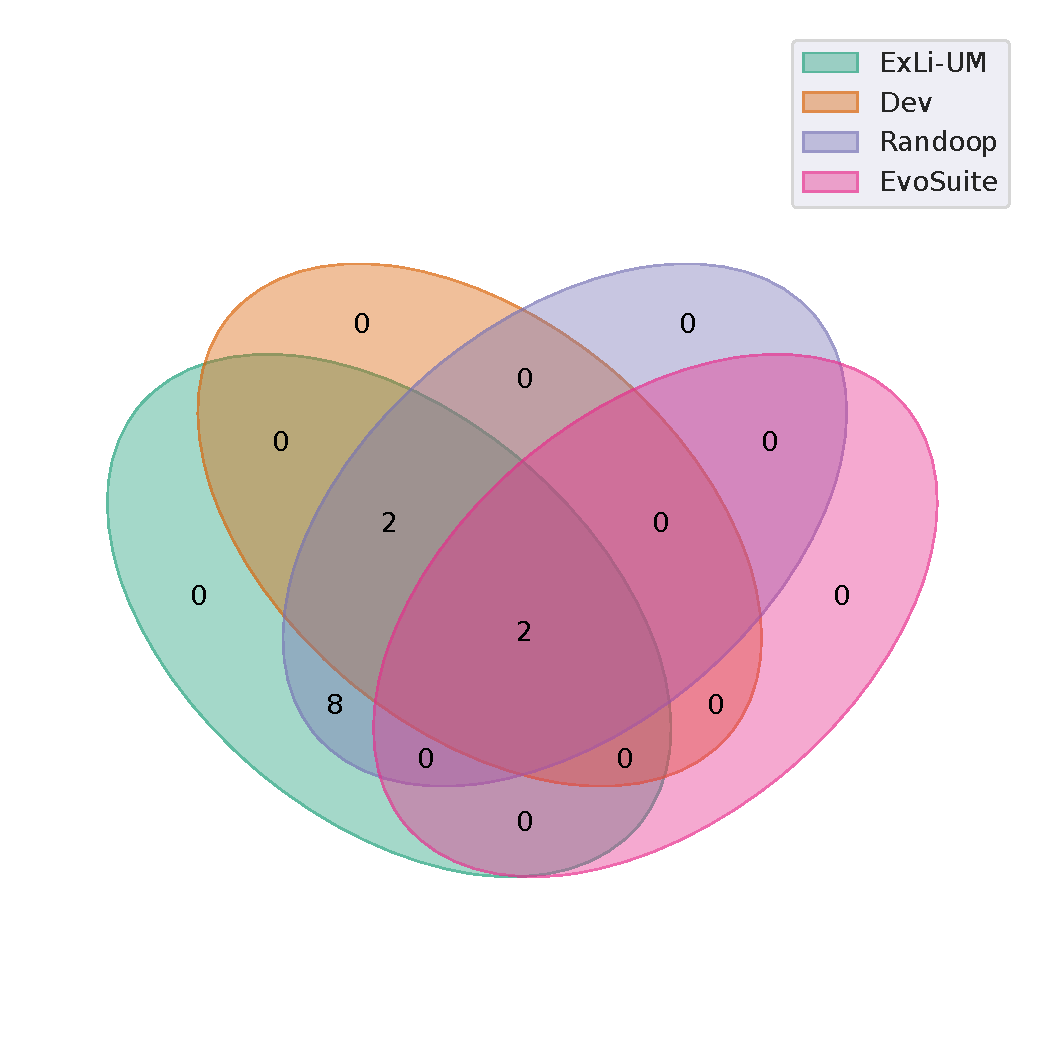
\includegraphics[width=\textwidth]{figures/venn/visenze_visearch-sdk-java-venn.pdf}
\vspace{-10pt}
\caption{visearch-sdk-java}
\label{fig:venn-visenze_visearch-sdk-java}
\end{subfigure}
\hfill
\begin{subfigure}[b]{0.45\textwidth}
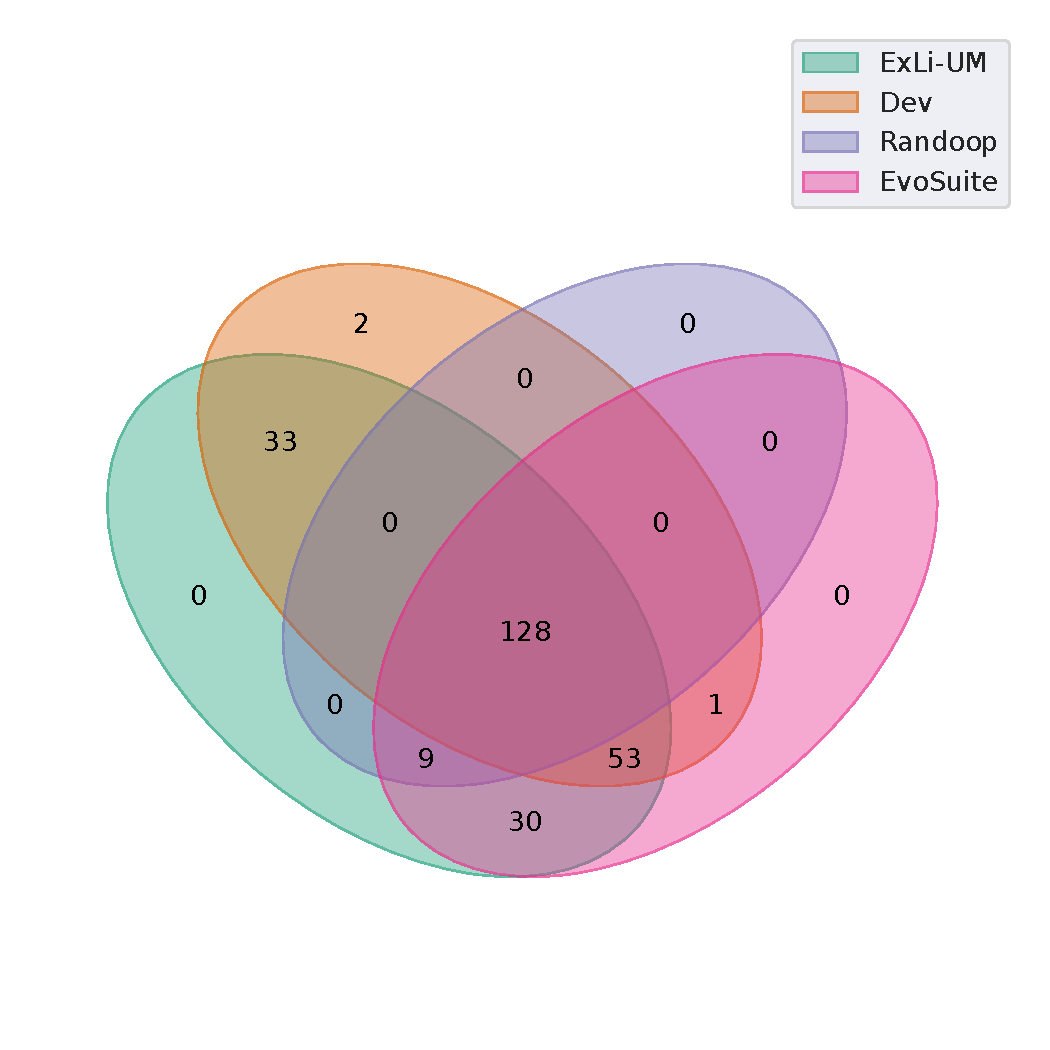
\includegraphics[width=\textwidth]{figures/venn/wmixvideo_nfe-venn.pdf}
\vspace{-10pt}
\caption{nfe}
\label{fig:venn-wmixvideo_nfe}
\end{subfigure}
\caption{Sets of mutants killed by inline tests and unit tests.}
\label{fig:venn-all}
\end{figure}